%% Manuscript for Computer Networks (Elsevier) -- elsarticle, numbered references.
%% Every number in the text is a macro \val{key} generated by scripts/r7_paper_assets.py
%% from the result files; do not type numbers by hand.
\documentclass[preprint,12pt]{elsarticle}

\usepackage[T1]{fontenc}
\usepackage{lmodern}
\usepackage{amsmath,amssymb}
\usepackage{graphicx}
\usepackage{booktabs}
\usepackage{multirow}
\usepackage{adjustbox}
\usepackage{array}
\usepackage{xcolor}
\usepackage{tikz}
\usetikzlibrary{arrows.meta,positioning,fit,calc}
\usepackage[hidelinks]{hyperref}
\usepackage{lineno}
\linenumbers

% generated by scripts/r7_paper_assets.py -- do not edit
\makeatletter
\@namedef{val@all.in.max}{1.000}
\@namedef{val@all.in.min}{0.939}
\@namedef{val@audit.BOT.dupall}{0.3\%}
\@namedef{val@audit.BOT.dupnoid}{99.7\%}
\@namedef{val@audit.BOT.dupnoiddns}{99.7\%}
\@namedef{val@audit.BOT.raw}{37{,}763{,}497}
\@namedef{val@audit.BOT.unoid}{101{,}369}
\@namedef{val@audit.BOT.unoiddns}{95{,}718}
\@namedef{val@audit.CIC.dupall}{0.0\%}
\@namedef{val@audit.CIC.dupnoid}{52.5\%}
\@namedef{val@audit.CIC.dupnoiddns}{89.5\%}
\@namedef{val@audit.CIC.raw}{18{,}893{,}708}
\@namedef{val@audit.CIC.unoid}{8{,}983{,}675}
\@namedef{val@audit.CIC.unoiddns}{1{,}980{,}571}
\@namedef{val@audit.TON.dupall}{0.0\%}
\@namedef{val@audit.TON.dupnoid}{85.4\%}
\@namedef{val@audit.TON.dupnoiddns}{93.8\%}
\@namedef{val@audit.TON.raw}{16{,}940{,}496}
\@namedef{val@audit.TON.unoid}{2{,}477{,}944}
\@namedef{val@audit.TON.unoiddns}{1{,}054{,}278}
\@namedef{val@audit.UN.dupall}{0.0\%}
\@namedef{val@audit.UN.dupnoid}{89.9\%}
\@namedef{val@audit.UN.dupnoiddns}{95.5\%}
\@namedef{val@audit.UN.raw}{2{,}390{,}275}
\@namedef{val@audit.UN.unoid}{241{,}206}
\@namedef{val@audit.UN.unoiddns}{108{,}243}
\@namedef{val@audit.dupall.max}{0.3\%}
\@namedef{val@v2bin.below.total}{21}
\@namedef{val@v2bin.cl.qmap-base.nclus}{8}
\@namedef{val@v2bin.cl.qmap-base.npairs}{12}
\@namedef{val@v2bin.cl.qmap-base.pmed}{-0.002}
\@namedef{val@v2bin.cl.qmap-base.pp}{0.733}
\@namedef{val@v2bin.cl.qmap-base.ppos}{6}
\@namedef{val@v2bin.cl.qmap-base.prrb}{-0.13}
\@namedef{val@v2bin.cl.qmap-base.rhi}{0.111}
\@namedef{val@v2bin.cl.qmap-base.rlo}{0.009}
\@namedef{val@v2bin.cl.qmap-base.rmean}{0.055}
\@namedef{val@v2bin.cl.qmapflip-base.nclus}{8}
\@namedef{val@v2bin.cl.qmapflip-base.npairs}{12}
\@namedef{val@v2bin.cl.qmapflip-base.pmed}{0.345}
\@namedef{val@v2bin.cl.qmapflip-base.pp}{0.010}
\@namedef{val@v2bin.cl.qmapflip-base.ppos}{10}
\@namedef{val@v2bin.cl.qmapflip-base.prrb}{0.87}
\@namedef{val@v2bin.cl.qmapflip-base.rhi}{0.510}
\@namedef{val@v2bin.cl.qmapflip-base.rlo}{0.367}
\@namedef{val@v2bin.cl.qmapflip-base.rmean}{0.439}
\@namedef{val@v2bin.cl.qmapflip-qmap.nclus}{8}
\@namedef{val@v2bin.cl.qmapflip-qmap.npairs}{12}
\@namedef{val@v2bin.cl.qmapflip-qmap.pmed}{0.311}
\@namedef{val@v2bin.cl.qmapflip-qmap.pp}{0.003}
\@namedef{val@v2bin.cl.qmapflip-qmap.ppos}{11}
\@namedef{val@v2bin.cl.qmapflip-qmap.prrb}{0.97}
\@namedef{val@v2bin.cl.qmapflip-qmap.rhi}{0.491}
\@namedef{val@v2bin.cl.qmapflip-qmap.rlo}{0.277}
\@namedef{val@v2bin.cl.qmapflip-qmap.rmean}{0.384}
\@namedef{val@v2bin.cl.qmapflip-randflip.nclus}{8}
\@namedef{val@v2bin.cl.qmapflip-randflip.npairs}{12}
\@namedef{val@v2bin.cl.qmapflip-randflip.pmed}{0.409}
\@namedef{val@v2bin.cl.qmapflip-randflip.pp}{0.002}
\@namedef{val@v2bin.cl.qmapflip-randflip.ppos}{12}
\@namedef{val@v2bin.cl.qmapflip-randflip.prrb}{1.00}
\@namedef{val@v2bin.cl.qmapflip-randflip.rhi}{0.507}
\@namedef{val@v2bin.cl.qmapflip-randflip.rlo}{0.381}
\@namedef{val@v2bin.cl.qmapflip-randflip.rmean}{0.453}
\@namedef{val@v2bin.cross.min}{0.155}
\@namedef{val@v2bin.f.nfeat}{38}
\@namedef{val@v2bin.f.nrevany}{30}
\@namedef{val@v2bin.f.prmax}{84.0\%}
\@namedef{val@v2bin.f.prmin}{41.7\%}
\@namedef{val@v2bin.f.rho}{-0.03}
\@namedef{val@v2bin.f.rhop}{0.931}
\@namedef{val@v2bin.fa.CLIENT_TCP_FLAGS.BOT}{0.703}
\@namedef{val@v2bin.fa.CLIENT_TCP_FLAGS.CIC}{0.381}
\@namedef{val@v2bin.fa.CLIENT_TCP_FLAGS.TON}{0.704}
\@namedef{val@v2bin.fa.CLIENT_TCP_FLAGS.UN}{0.383}
\@namedef{val@v2bin.fa.DNS_QUERY_TYPE.BOT}{0.467}
\@namedef{val@v2bin.fa.DNS_QUERY_TYPE.CIC}{0.461}
\@namedef{val@v2bin.fa.DNS_QUERY_TYPE.TON}{0.363}
\@namedef{val@v2bin.fa.DNS_QUERY_TYPE.UN}{0.501}
\@namedef{val@v2bin.fa.DNS_TTL_ANSWER.BOT}{0.468}
\@namedef{val@v2bin.fa.DNS_TTL_ANSWER.CIC}{0.462}
\@namedef{val@v2bin.fa.DNS_TTL_ANSWER.TON}{0.398}
\@namedef{val@v2bin.fa.DNS_TTL_ANSWER.UN}{0.500}
\@namedef{val@v2bin.fa.DST_TO_SRC_AVG_THROUGHPUT.BOT}{0.526}
\@namedef{val@v2bin.fa.DST_TO_SRC_AVG_THROUGHPUT.CIC}{0.106}
\@namedef{val@v2bin.fa.DST_TO_SRC_AVG_THROUGHPUT.TON}{0.566}
\@namedef{val@v2bin.fa.DST_TO_SRC_AVG_THROUGHPUT.UN}{0.341}
\@namedef{val@v2bin.fa.DST_TO_SRC_SECOND_BYTES.BOT}{0.415}
\@namedef{val@v2bin.fa.DST_TO_SRC_SECOND_BYTES.CIC}{0.629}
\@namedef{val@v2bin.fa.DST_TO_SRC_SECOND_BYTES.TON}{0.752}
\@namedef{val@v2bin.fa.DST_TO_SRC_SECOND_BYTES.UN}{0.294}
\@namedef{val@v2bin.fa.DURATION_IN.BOT}{0.501}
\@namedef{val@v2bin.fa.DURATION_IN.CIC}{0.959}
\@namedef{val@v2bin.fa.DURATION_IN.TON}{0.634}
\@namedef{val@v2bin.fa.DURATION_IN.UN}{0.412}
\@namedef{val@v2bin.fa.DURATION_OUT.BOT}{0.383}
\@namedef{val@v2bin.fa.DURATION_OUT.CIC}{0.937}
\@namedef{val@v2bin.fa.DURATION_OUT.TON}{0.732}
\@namedef{val@v2bin.fa.DURATION_OUT.UN}{0.411}
\@namedef{val@v2bin.fa.FLOW_DURATION_MILLISECONDS.BOT}{0.626}
\@namedef{val@v2bin.fa.FLOW_DURATION_MILLISECONDS.CIC}{0.728}
\@namedef{val@v2bin.fa.FLOW_DURATION_MILLISECONDS.TON}{0.650}
\@namedef{val@v2bin.fa.FLOW_DURATION_MILLISECONDS.UN}{0.422}
\@namedef{val@v2bin.fa.FTP_COMMAND_RET_CODE.BOT}{0.501}
\@namedef{val@v2bin.fa.FTP_COMMAND_RET_CODE.CIC}{0.500}
\@namedef{val@v2bin.fa.FTP_COMMAND_RET_CODE.TON}{0.501}
\@namedef{val@v2bin.fa.FTP_COMMAND_RET_CODE.UN}{0.498}
\@namedef{val@v2bin.fa.ICMP_IPV4_TYPE.BOT}{0.620}
\@namedef{val@v2bin.fa.ICMP_IPV4_TYPE.CIC}{0.528}
\@namedef{val@v2bin.fa.ICMP_IPV4_TYPE.TON}{0.473}
\@namedef{val@v2bin.fa.ICMP_IPV4_TYPE.UN}{0.542}
\@namedef{val@v2bin.fa.ICMP_TYPE.BOT}{0.620}
\@namedef{val@v2bin.fa.ICMP_TYPE.CIC}{0.528}
\@namedef{val@v2bin.fa.ICMP_TYPE.TON}{0.473}
\@namedef{val@v2bin.fa.ICMP_TYPE.UN}{0.542}
\@namedef{val@v2bin.fa.IN_BYTES.BOT}{0.329}
\@namedef{val@v2bin.fa.IN_BYTES.CIC}{0.635}
\@namedef{val@v2bin.fa.IN_BYTES.TON}{0.682}
\@namedef{val@v2bin.fa.IN_BYTES.UN}{0.331}
\@namedef{val@v2bin.fa.IN_PKTS.BOT}{0.356}
\@namedef{val@v2bin.fa.IN_PKTS.CIC}{0.602}
\@namedef{val@v2bin.fa.IN_PKTS.TON}{0.706}
\@namedef{val@v2bin.fa.IN_PKTS.UN}{0.276}
\@namedef{val@v2bin.fa.L7_PROTO.BOT}{0.661}
\@namedef{val@v2bin.fa.L7_PROTO.CIC}{0.542}
\@namedef{val@v2bin.fa.L7_PROTO.TON}{0.599}
\@namedef{val@v2bin.fa.L7_PROTO.UN}{0.600}
\@namedef{val@v2bin.fa.LONGEST_FLOW_PKT.BOT}{0.297}
\@namedef{val@v2bin.fa.LONGEST_FLOW_PKT.CIC}{0.286}
\@namedef{val@v2bin.fa.LONGEST_FLOW_PKT.TON}{0.769}
\@namedef{val@v2bin.fa.LONGEST_FLOW_PKT.UN}{0.462}
\@namedef{val@v2bin.fa.MAX_IP_PKT_LEN.BOT}{0.297}
\@namedef{val@v2bin.fa.MAX_IP_PKT_LEN.CIC}{0.286}
\@namedef{val@v2bin.fa.MAX_IP_PKT_LEN.TON}{0.769}
\@namedef{val@v2bin.fa.MAX_IP_PKT_LEN.UN}{0.462}
\@namedef{val@v2bin.fa.MAX_TTL.BOT}{0.335}
\@namedef{val@v2bin.fa.MAX_TTL.CIC}{0.168}
\@namedef{val@v2bin.fa.MAX_TTL.TON}{0.590}
\@namedef{val@v2bin.fa.MAX_TTL.UN}{0.875}
\@namedef{val@v2bin.fa.MIN_IP_PKT_LEN.BOT}{0.491}
\@namedef{val@v2bin.fa.MIN_IP_PKT_LEN.CIC}{0.764}
\@namedef{val@v2bin.fa.MIN_IP_PKT_LEN.TON}{0.460}
\@namedef{val@v2bin.fa.MIN_IP_PKT_LEN.UN}{0.138}
\@namedef{val@v2bin.fa.MIN_TTL.BOT}{0.334}
\@namedef{val@v2bin.fa.MIN_TTL.CIC}{0.169}
\@namedef{val@v2bin.fa.MIN_TTL.TON}{0.593}
\@namedef{val@v2bin.fa.MIN_TTL.UN}{0.873}
\@namedef{val@v2bin.fa.NUM_PKTS_1024_TO_1514_BYTES.BOT}{0.295}
\@namedef{val@v2bin.fa.NUM_PKTS_1024_TO_1514_BYTES.CIC}{0.173}
\@namedef{val@v2bin.fa.NUM_PKTS_1024_TO_1514_BYTES.TON}{0.705}
\@namedef{val@v2bin.fa.NUM_PKTS_1024_TO_1514_BYTES.UN}{0.369}
\@namedef{val@v2bin.fa.NUM_PKTS_128_TO_256_BYTES.BOT}{0.653}
\@namedef{val@v2bin.fa.NUM_PKTS_128_TO_256_BYTES.CIC}{0.124}
\@namedef{val@v2bin.fa.NUM_PKTS_128_TO_256_BYTES.TON}{0.511}
\@namedef{val@v2bin.fa.NUM_PKTS_128_TO_256_BYTES.UN}{0.599}
\@namedef{val@v2bin.fa.NUM_PKTS_256_TO_512_BYTES.BOT}{0.249}
\@namedef{val@v2bin.fa.NUM_PKTS_256_TO_512_BYTES.CIC}{0.714}
\@namedef{val@v2bin.fa.NUM_PKTS_256_TO_512_BYTES.TON}{0.675}
\@namedef{val@v2bin.fa.NUM_PKTS_256_TO_512_BYTES.UN}{0.397}
\@namedef{val@v2bin.fa.NUM_PKTS_512_TO_1024_BYTES.BOT}{0.318}
\@namedef{val@v2bin.fa.NUM_PKTS_512_TO_1024_BYTES.CIC}{0.779}
\@namedef{val@v2bin.fa.NUM_PKTS_512_TO_1024_BYTES.TON}{0.635}
\@namedef{val@v2bin.fa.NUM_PKTS_512_TO_1024_BYTES.UN}{0.431}
\@namedef{val@v2bin.fa.NUM_PKTS_UP_TO_128_BYTES.BOT}{0.614}
\@namedef{val@v2bin.fa.NUM_PKTS_UP_TO_128_BYTES.CIC}{0.622}
\@namedef{val@v2bin.fa.NUM_PKTS_UP_TO_128_BYTES.TON}{0.687}
\@namedef{val@v2bin.fa.NUM_PKTS_UP_TO_128_BYTES.UN}{0.257}
\@namedef{val@v2bin.fa.OUT_BYTES.BOT}{0.463}
\@namedef{val@v2bin.fa.OUT_BYTES.CIC}{0.449}
\@namedef{val@v2bin.fa.OUT_BYTES.TON}{0.811}
\@namedef{val@v2bin.fa.OUT_BYTES.UN}{0.293}
\@namedef{val@v2bin.fa.OUT_PKTS.BOT}{0.482}
\@namedef{val@v2bin.fa.OUT_PKTS.CIC}{0.518}
\@namedef{val@v2bin.fa.OUT_PKTS.TON}{0.780}
\@namedef{val@v2bin.fa.OUT_PKTS.UN}{0.266}
\@namedef{val@v2bin.fa.PROTOCOL.BOT}{0.388}
\@namedef{val@v2bin.fa.PROTOCOL.CIC}{0.477}
\@namedef{val@v2bin.fa.PROTOCOL.TON}{0.383}
\@namedef{val@v2bin.fa.PROTOCOL.UN}{0.536}
\@namedef{val@v2bin.fa.RETRANSMITTED_IN_BYTES.BOT}{0.597}
\@namedef{val@v2bin.fa.RETRANSMITTED_IN_BYTES.CIC}{0.569}
\@namedef{val@v2bin.fa.RETRANSMITTED_IN_BYTES.TON}{0.494}
\@namedef{val@v2bin.fa.RETRANSMITTED_IN_BYTES.UN}{0.369}
\@namedef{val@v2bin.fa.RETRANSMITTED_IN_PKTS.BOT}{0.597}
\@namedef{val@v2bin.fa.RETRANSMITTED_IN_PKTS.CIC}{0.517}
\@namedef{val@v2bin.fa.RETRANSMITTED_IN_PKTS.TON}{0.492}
\@namedef{val@v2bin.fa.RETRANSMITTED_IN_PKTS.UN}{0.337}
\@namedef{val@v2bin.fa.RETRANSMITTED_OUT_BYTES.BOT}{0.447}
\@namedef{val@v2bin.fa.RETRANSMITTED_OUT_BYTES.CIC}{0.544}
\@namedef{val@v2bin.fa.RETRANSMITTED_OUT_BYTES.TON}{0.606}
\@namedef{val@v2bin.fa.RETRANSMITTED_OUT_BYTES.UN}{0.310}
\@namedef{val@v2bin.fa.RETRANSMITTED_OUT_PKTS.BOT}{0.447}
\@namedef{val@v2bin.fa.RETRANSMITTED_OUT_PKTS.CIC}{0.531}
\@namedef{val@v2bin.fa.RETRANSMITTED_OUT_PKTS.TON}{0.606}
\@namedef{val@v2bin.fa.RETRANSMITTED_OUT_PKTS.UN}{0.290}
\@namedef{val@v2bin.fa.SERVER_TCP_FLAGS.BOT}{0.764}
\@namedef{val@v2bin.fa.SERVER_TCP_FLAGS.CIC}{0.523}
\@namedef{val@v2bin.fa.SERVER_TCP_FLAGS.TON}{0.866}
\@namedef{val@v2bin.fa.SERVER_TCP_FLAGS.UN}{0.176}
\@namedef{val@v2bin.fa.SHORTEST_FLOW_PKT.BOT}{0.268}
\@namedef{val@v2bin.fa.SHORTEST_FLOW_PKT.CIC}{0.781}
\@namedef{val@v2bin.fa.SHORTEST_FLOW_PKT.TON}{0.401}
\@namedef{val@v2bin.fa.SHORTEST_FLOW_PKT.UN}{0.218}
\@namedef{val@v2bin.fa.SRC_TO_DST_AVG_THROUGHPUT.BOT}{0.337}
\@namedef{val@v2bin.fa.SRC_TO_DST_AVG_THROUGHPUT.CIC}{0.069}
\@namedef{val@v2bin.fa.SRC_TO_DST_AVG_THROUGHPUT.TON}{0.531}
\@namedef{val@v2bin.fa.SRC_TO_DST_AVG_THROUGHPUT.UN}{0.445}
\@namedef{val@v2bin.fa.SRC_TO_DST_SECOND_BYTES.BOT}{0.384}
\@namedef{val@v2bin.fa.SRC_TO_DST_SECOND_BYTES.CIC}{0.770}
\@namedef{val@v2bin.fa.SRC_TO_DST_SECOND_BYTES.TON}{0.632}
\@namedef{val@v2bin.fa.SRC_TO_DST_SECOND_BYTES.UN}{0.329}
\@namedef{val@v2bin.fa.TCP_FLAGS.BOT}{0.749}
\@namedef{val@v2bin.fa.TCP_FLAGS.CIC}{0.351}
\@namedef{val@v2bin.fa.TCP_FLAGS.TON}{0.712}
\@namedef{val@v2bin.fa.TCP_FLAGS.UN}{0.373}
\@namedef{val@v2bin.fa.TCP_WIN_MAX_IN.BOT}{0.522}
\@namedef{val@v2bin.fa.TCP_WIN_MAX_IN.CIC}{0.841}
\@namedef{val@v2bin.fa.TCP_WIN_MAX_IN.TON}{0.823}
\@namedef{val@v2bin.fa.TCP_WIN_MAX_IN.UN}{0.235}
\@namedef{val@v2bin.fa.TCP_WIN_MAX_OUT.BOT}{0.664}
\@namedef{val@v2bin.fa.TCP_WIN_MAX_OUT.CIC}{0.269}
\@namedef{val@v2bin.fa.TCP_WIN_MAX_OUT.TON}{0.744}
\@namedef{val@v2bin.fa.TCP_WIN_MAX_OUT.UN}{0.427}
\@namedef{val@v2bin.few.100.est}{0.737}
\@namedef{val@v2bin.few.100.hi}{0.786}
\@namedef{val@v2bin.few.100.lo}{0.686}
\@namedef{val@v2bin.few.100.oracle}{0.739}
\@namedef{val@v2bin.few.100.prec}{0.94}
\@namedef{val@v2bin.few.100.rec}{0.93}
\@namedef{val@v2bin.few.100.tolr}{0.941}
\@namedef{val@v2bin.few.100.toxgb}{0.963}
\@namedef{val@v2bin.few.20.est}{0.727}
\@namedef{val@v2bin.few.20.hi}{0.777}
\@namedef{val@v2bin.few.20.lo}{0.675}
\@namedef{val@v2bin.few.20.oracle}{0.739}
\@namedef{val@v2bin.few.20.prec}{0.86}
\@namedef{val@v2bin.few.20.rec}{0.82}
\@namedef{val@v2bin.few.20.tolr}{0.835}
\@namedef{val@v2bin.few.20.toxgb}{0.877}
\@namedef{val@v2bin.few.200.est}{0.738}
\@namedef{val@v2bin.few.200.hi}{0.788}
\@namedef{val@v2bin.few.200.lo}{0.687}
\@namedef{val@v2bin.few.200.oracle}{0.739}
\@namedef{val@v2bin.few.200.prec}{0.96}
\@namedef{val@v2bin.few.200.rec}{0.96}
\@namedef{val@v2bin.few.200.tolr}{0.954}
\@namedef{val@v2bin.few.200.toxgb}{0.974}
\@namedef{val@v2bin.few.50.est}{0.734}
\@namedef{val@v2bin.few.50.hi}{0.783}
\@namedef{val@v2bin.few.50.lo}{0.682}
\@namedef{val@v2bin.few.50.oracle}{0.739}
\@namedef{val@v2bin.few.50.prec}{0.91}
\@namedef{val@v2bin.few.50.rec}{0.90}
\@namedef{val@v2bin.few.50.tolr}{0.905}
\@namedef{val@v2bin.few.50.toxgb}{0.942}
\@namedef{val@v2bin.few.500.est}{0.740}
\@namedef{val@v2bin.few.500.hi}{0.790}
\@namedef{val@v2bin.few.500.lo}{0.689}
\@namedef{val@v2bin.few.500.oracle}{0.739}
\@namedef{val@v2bin.few.500.prec}{0.98}
\@namedef{val@v2bin.few.500.rec}{0.98}
\@namedef{val@v2bin.few.500.tolr}{0.963}
\@namedef{val@v2bin.few.500.toxgb}{0.982}
\@namedef{val@v2bin.few.nrev}{19}
\@namedef{val@v2bin.fr.CLIENT_TCP_FLAGS}{4}
\@namedef{val@v2bin.fr.DNS_QUERY_TYPE}{0}
\@namedef{val@v2bin.fr.DNS_TTL_ANSWER}{0}
\@namedef{val@v2bin.fr.DST_TO_SRC_AVG_THROUGHPUT}{2}
\@namedef{val@v2bin.fr.DST_TO_SRC_SECOND_BYTES}{4}
\@namedef{val@v2bin.fr.DURATION_IN}{2}
\@namedef{val@v2bin.fr.DURATION_OUT}{4}
\@namedef{val@v2bin.fr.FLOW_DURATION_MILLISECONDS}{3}
\@namedef{val@v2bin.fr.FTP_COMMAND_RET_CODE}{0}
\@namedef{val@v2bin.fr.ICMP_IPV4_TYPE}{0}
\@namedef{val@v2bin.fr.ICMP_TYPE}{0}
\@namedef{val@v2bin.fr.IN_BYTES}{4}
\@namedef{val@v2bin.fr.IN_PKTS}{4}
\@namedef{val@v2bin.fr.L7_PROTO}{0}
\@namedef{val@v2bin.fr.LONGEST_FLOW_PKT}{2}
\@namedef{val@v2bin.fr.MAX_IP_PKT_LEN}{2}
\@namedef{val@v2bin.fr.MAX_TTL}{4}
\@namedef{val@v2bin.fr.MIN_IP_PKT_LEN}{1}
\@namedef{val@v2bin.fr.MIN_TTL}{4}
\@namedef{val@v2bin.fr.NUM_PKTS_1024_TO_1514_BYTES}{3}
\@namedef{val@v2bin.fr.NUM_PKTS_128_TO_256_BYTES}{2}
\@namedef{val@v2bin.fr.NUM_PKTS_256_TO_512_BYTES}{4}
\@namedef{val@v2bin.fr.NUM_PKTS_512_TO_1024_BYTES}{4}
\@namedef{val@v2bin.fr.NUM_PKTS_UP_TO_128_BYTES}{3}
\@namedef{val@v2bin.fr.OUT_BYTES}{2}
\@namedef{val@v2bin.fr.OUT_PKTS}{1}
\@namedef{val@v2bin.fr.PROTOCOL}{0}
\@namedef{val@v2bin.fr.RETRANSMITTED_IN_BYTES}{2}
\@namedef{val@v2bin.fr.RETRANSMITTED_IN_PKTS}{1}
\@namedef{val@v2bin.fr.RETRANSMITTED_OUT_BYTES}{2}
\@namedef{val@v2bin.fr.RETRANSMITTED_OUT_PKTS}{2}
\@namedef{val@v2bin.fr.SERVER_TCP_FLAGS}{2}
\@namedef{val@v2bin.fr.SHORTEST_FLOW_PKT}{3}
\@namedef{val@v2bin.fr.SRC_TO_DST_AVG_THROUGHPUT}{0}
\@namedef{val@v2bin.fr.SRC_TO_DST_SECOND_BYTES}{4}
\@namedef{val@v2bin.fr.TCP_FLAGS}{4}
\@namedef{val@v2bin.fr.TCP_WIN_MAX_IN}{2}
\@namedef{val@v2bin.fr.TCP_WIN_MAX_OUT}{4}
\@namedef{val@v2bin.in.max}{0.998}
\@namedef{val@v2bin.in.min}{0.939}
\@namedef{val@v2bin.lodo.below}{3}
\@namedef{val@v2bin.lodo.min}{0.231}
\@namedef{val@v2bin.lodo.n}{12}
\@namedef{val@v2bin.lr.BOT.BOT}{0.991}
\@namedef{val@v2bin.lr.BOT.CIC}{0.589}
\@namedef{val@v2bin.lr.BOT.TON}{0.649}
\@namedef{val@v2bin.lr.BOT.UN}{0.458}
\@namedef{val@v2bin.lr.CIC.BOT}{0.365}
\@namedef{val@v2bin.lr.CIC.CIC}{0.989}
\@namedef{val@v2bin.lr.CIC.TON}{0.653}
\@namedef{val@v2bin.lr.CIC.UN}{0.258}
\@namedef{val@v2bin.lr.TON.BOT}{0.432}
\@namedef{val@v2bin.lr.TON.CIC}{0.822}
\@namedef{val@v2bin.lr.TON.TON}{0.939}
\@namedef{val@v2bin.lr.TON.UN}{0.284}
\@namedef{val@v2bin.lr.UN.BOT}{0.285}
\@namedef{val@v2bin.lr.UN.CIC}{0.277}
\@namedef{val@v2bin.lr.UN.TON}{0.338}
\@namedef{val@v2bin.lr.UN.UN}{0.957}
\@namedef{val@v2bin.lr.below}{8}
\@namedef{val@v2bin.lr.crossmean}{0.451}
\@namedef{val@v2bin.lr.inmean}{0.969}
\@namedef{val@v2bin.lr.min}{0.258}
\@namedef{val@v2bin.lr.mincell}{CIC$\rightarrow$UN}
\@namedef{val@v2bin.lr.rev}{7}
\@namedef{val@v2bin.lr.robust}{7}
\@namedef{val@v2bin.mlp.BOT.BOT}{0.998}
\@namedef{val@v2bin.mlp.BOT.CIC}{0.525}
\@namedef{val@v2bin.mlp.BOT.TON}{0.581}
\@namedef{val@v2bin.mlp.BOT.UN}{0.253}
\@namedef{val@v2bin.mlp.CIC.BOT}{0.409}
\@namedef{val@v2bin.mlp.CIC.CIC}{0.995}
\@namedef{val@v2bin.mlp.CIC.TON}{0.605}
\@namedef{val@v2bin.mlp.CIC.UN}{0.273}
\@namedef{val@v2bin.mlp.TON.BOT}{0.844}
\@namedef{val@v2bin.mlp.TON.CIC}{0.782}
\@namedef{val@v2bin.mlp.TON.TON}{0.989}
\@namedef{val@v2bin.mlp.TON.UN}{0.438}
\@namedef{val@v2bin.mlp.UN.BOT}{0.155}
\@namedef{val@v2bin.mlp.UN.CIC}{0.302}
\@namedef{val@v2bin.mlp.UN.TON}{0.257}
\@namedef{val@v2bin.mlp.UN.UN}{0.982}
\@namedef{val@v2bin.mlp.below}{7}
\@namedef{val@v2bin.mlp.crossmean}{0.452}
\@namedef{val@v2bin.mlp.inmean}{0.991}
\@namedef{val@v2bin.mlp.min}{0.155}
\@namedef{val@v2bin.mlp.mincell}{UN$\rightarrow$BOT}
\@namedef{val@v2bin.mlp.rev}{7}
\@namedef{val@v2bin.mlp.robust}{5}
\@namedef{val@v2bin.ncells}{36}
\@namedef{val@v2bin.nfeat}{38}
\@namedef{val@v2bin.or.all.base}{0.470}
\@namedef{val@v2bin.or.all.flip}{0.638}
\@namedef{val@v2bin.or.all.qmap}{0.452}
\@namedef{val@v2bin.or.all.qmapflip}{0.733}
\@namedef{val@v2bin.or.all.randflip}{0.297}
\@namedef{val@v2bin.or.nall}{36}
\@namedef{val@v2bin.or.nflip.max}{21}
\@namedef{val@v2bin.or.nflip.mean}{14.2}
\@namedef{val@v2bin.or.nflip.min}{10}
\@namedef{val@v2bin.or.nrev}{19}
\@namedef{val@v2bin.or.rest.base}{0}
\@namedef{val@v2bin.or.rest.flip}{14}
\@namedef{val@v2bin.or.rest.qmap}{3}
\@namedef{val@v2bin.or.rest.qmapflip}{17}
\@namedef{val@v2bin.or.rest.randflip}{2}
\@namedef{val@v2bin.or.rev.base}{0.300}
\@namedef{val@v2bin.or.rev.base.hi}{0.336}
\@namedef{val@v2bin.or.rev.base.lo}{0.265}
\@namedef{val@v2bin.or.rev.flip}{0.649}
\@namedef{val@v2bin.or.rev.flip.hi}{0.729}
\@namedef{val@v2bin.or.rev.flip.lo}{0.558}
\@namedef{val@v2bin.or.rev.qmap}{0.355}
\@namedef{val@v2bin.or.rev.qmap.hi}{0.419}
\@namedef{val@v2bin.or.rev.qmap.lo}{0.298}
\@namedef{val@v2bin.or.rev.qmapflip}{0.739}
\@namedef{val@v2bin.or.rev.qmapflip.hi}{0.791}
\@namedef{val@v2bin.or.rev.qmapflip.lo}{0.687}
\@namedef{val@v2bin.or.rev.randflip}{0.285}
\@namedef{val@v2bin.or.rev.randflip.hi}{0.346}
\@namedef{val@v2bin.or.rev.randflip.lo}{0.233}
\@namedef{val@v2bin.pos.BOT.CIC.ta}{0.697}
\@namedef{val@v2bin.pos.BOT.CIC.tb}{0.457}
\@namedef{val@v2bin.pos.BOT.TON.ta}{0.891}
\@namedef{val@v2bin.pos.BOT.TON.tb}{0.377}
\@namedef{val@v2bin.pos.BOT.UN.ta}{0.165}
\@namedef{val@v2bin.pos.BOT.UN.tb}{0.445}
\@namedef{val@v2bin.pos.CIC.BOT.ta}{0.102}
\@namedef{val@v2bin.pos.CIC.BOT.tb}{0.392}
\@namedef{val@v2bin.pos.CIC.TON.ta}{0.410}
\@namedef{val@v2bin.pos.CIC.TON.tb}{0.194}
\@namedef{val@v2bin.pos.CIC.UN.ta}{0.010}
\@namedef{val@v2bin.pos.CIC.UN.tb}{0.056}
\@namedef{val@v2bin.pos.TON.BOT.ta}{0.151}
\@namedef{val@v2bin.pos.TON.BOT.tb}{0.052}
\@namedef{val@v2bin.pos.TON.CIC.ta}{0.528}
\@namedef{val@v2bin.pos.TON.CIC.tb}{0.001}
\@namedef{val@v2bin.pos.TON.UN.ta}{0.013}
\@namedef{val@v2bin.pos.TON.UN.tb}{0.191}
\@namedef{val@v2bin.pos.UN.BOT.ta}{0.014}
\@namedef{val@v2bin.pos.UN.BOT.tb}{0.236}
\@namedef{val@v2bin.pos.UN.CIC.ta}{0.005}
\@namedef{val@v2bin.pos.UN.CIC.tb}{0.385}
\@namedef{val@v2bin.pos.UN.TON.ta}{0.007}
\@namedef{val@v2bin.pos.UN.TON.tb}{0.064}
\@namedef{val@v2bin.pos.coll}{0}
\@namedef{val@v2bin.pos.inv}{7}
\@namedef{val@v2bin.pos.n}{12}
\@namedef{val@v2bin.rev.total}{19}
\@namedef{val@v2bin.robust.total}{16}
\@namedef{val@v2bin.sens.restmax}{19}
\@namedef{val@v2bin.sens.restmin}{17}
\@namedef{val@v2bin.sens.rfmax}{3}
\@namedef{val@v2bin.st.BOT.ben}{15{,}569}
\@namedef{val@v2bin.st.BOT.nan}{0}
\@namedef{val@v2bin.st.BOT.pos}{80{,}149}
\@namedef{val@v2bin.st.BOT.raw}{37{,}763{,}497}
\@namedef{val@v2bin.st.BOT.uniq}{95{,}718}
\@namedef{val@v2bin.st.CIC.ben}{1{,}488{,}196}
\@namedef{val@v2bin.st.CIC.nan}{0}
\@namedef{val@v2bin.st.CIC.pos}{492{,}375}
\@namedef{val@v2bin.st.CIC.raw}{18{,}893{,}708}
\@namedef{val@v2bin.st.CIC.uniq}{1{,}980{,}571}
\@namedef{val@v2bin.st.TON.ben}{279{,}349}
\@namedef{val@v2bin.st.TON.nan}{0}
\@namedef{val@v2bin.st.TON.pos}{774{,}929}
\@namedef{val@v2bin.st.TON.raw}{16{,}940{,}496}
\@namedef{val@v2bin.st.TON.uniq}{1{,}054{,}278}
\@namedef{val@v2bin.st.UN.ben}{68{,}992}
\@namedef{val@v2bin.st.UN.nan}{0}
\@namedef{val@v2bin.st.UN.pos}{39{,}251}
\@namedef{val@v2bin.st.UN.raw}{2{,}390{,}275}
\@namedef{val@v2bin.st.UN.uniq}{108{,}243}
\@namedef{val@v2bin.swapattackside}{6}
\@namedef{val@v2bin.swapbenignside}{1}
\@namedef{val@v2bin.swapbothabove}{12}
\@namedef{val@v2bin.swaprevn}{19}
\@namedef{val@v2bin.t.all.qmap-base.med}{-0.005}
\@namedef{val@v2bin.t.all.qmap-base.n}{36}
\@namedef{val@v2bin.t.all.qmap-base.p}{0.647}
\@namedef{val@v2bin.t.all.qmap-base.rrb}{-0.09}
\@namedef{val@v2bin.t.all.qmapflip-base.med}{0.284}
\@namedef{val@v2bin.t.all.qmapflip-base.n}{36}
\@namedef{val@v2bin.t.all.qmapflip-base.p}{7.9\times10^{-6}}
\@namedef{val@v2bin.t.all.qmapflip-base.rrb}{0.81}
\@namedef{val@v2bin.t.all.qmapflip-qmap.med}{0.257}
\@namedef{val@v2bin.t.all.qmapflip-qmap.n}{36}
\@namedef{val@v2bin.t.all.qmapflip-qmap.p}{3.9\times10^{-8}}
\@namedef{val@v2bin.t.all.qmapflip-qmap.rrb}{0.94}
\@namedef{val@v2bin.t.all.qmapflip-randflip.med}{0.403}
\@namedef{val@v2bin.t.all.qmapflip-randflip.n}{36}
\@namedef{val@v2bin.t.all.qmapflip-randflip.p}{3.5\times10^{-10}}
\@namedef{val@v2bin.t.all.qmapflip-randflip.rrb}{0.99}
\@namedef{val@v2bin.t.rev.qmap-base.med}{0.037}
\@namedef{val@v2bin.t.rev.qmap-base.n}{19}
\@namedef{val@v2bin.t.rev.qmap-base.p}{0.040}
\@namedef{val@v2bin.t.rev.qmap-base.rrb}{0.54}
\@namedef{val@v2bin.t.rev.qmapflip-base.med}{0.474}
\@namedef{val@v2bin.t.rev.qmapflip-base.n}{19}
\@namedef{val@v2bin.t.rev.qmapflip-base.p}{1.5\times10^{-5}}
\@namedef{val@v2bin.t.rev.qmapflip-base.rrb}{1.00}
\@namedef{val@v2bin.t.rev.qmapflip-qmap.med}{0.402}
\@namedef{val@v2bin.t.rev.qmapflip-qmap.n}{19}
\@namedef{val@v2bin.t.rev.qmapflip-qmap.p}{1.5\times10^{-5}}
\@namedef{val@v2bin.t.rev.qmapflip-qmap.rrb}{1.00}
\@namedef{val@v2bin.t.rev.qmapflip-randflip.med}{0.406}
\@namedef{val@v2bin.t.rev.qmapflip-randflip.n}{19}
\@namedef{val@v2bin.t.rev.qmapflip-randflip.p}{1.5\times10^{-5}}
\@namedef{val@v2bin.t.rev.qmapflip-randflip.rrb}{1.00}
\@namedef{val@v2bin.xgboost.BOT.BOT}{0.998}
\@namedef{val@v2bin.xgboost.BOT.CIC}{0.882}
\@namedef{val@v2bin.xgboost.BOT.TON}{0.825}
\@namedef{val@v2bin.xgboost.BOT.UN}{0.346}
\@namedef{val@v2bin.xgboost.CIC.BOT}{0.385}
\@namedef{val@v2bin.xgboost.CIC.CIC}{0.996}
\@namedef{val@v2bin.xgboost.CIC.TON}{0.545}
\@namedef{val@v2bin.xgboost.CIC.UN}{0.631}
\@namedef{val@v2bin.xgboost.TON.BOT}{0.796}
\@namedef{val@v2bin.xgboost.TON.CIC}{0.554}
\@namedef{val@v2bin.xgboost.TON.TON}{0.995}
\@namedef{val@v2bin.xgboost.TON.UN}{0.478}
\@namedef{val@v2bin.xgboost.UN.BOT}{0.214}
\@namedef{val@v2bin.xgboost.UN.CIC}{0.166}
\@namedef{val@v2bin.xgboost.UN.TON}{0.269}
\@namedef{val@v2bin.xgboost.UN.UN}{0.985}
\@namedef{val@v2bin.xgboost.below}{6}
\@namedef{val@v2bin.xgboost.crossmean}{0.508}
\@namedef{val@v2bin.xgboost.inmean}{0.994}
\@namedef{val@v2bin.xgboost.min}{0.166}
\@namedef{val@v2bin.xgboost.mincell}{UN$\rightarrow$CIC}
\@namedef{val@v2bin.xgboost.rev}{5}
\@namedef{val@v2bin.xgboost.robust}{4}
\@namedef{val@v2dos.below.total}{20}
\@namedef{val@v2dos.cl.qmap-base.nclus}{8}
\@namedef{val@v2dos.cl.qmap-base.npairs}{12}
\@namedef{val@v2dos.cl.qmap-base.pmed}{-0.009}
\@namedef{val@v2dos.cl.qmap-base.pp}{0.622}
\@namedef{val@v2dos.cl.qmap-base.ppos}{5}
\@namedef{val@v2dos.cl.qmap-base.prrb}{-0.18}
\@namedef{val@v2dos.cl.qmap-base.rhi}{0.116}
\@namedef{val@v2dos.cl.qmap-base.rlo}{-0.025}
\@namedef{val@v2dos.cl.qmap-base.rmean}{0.042}
\@namedef{val@v2dos.cl.qmapflip-base.nclus}{8}
\@namedef{val@v2dos.cl.qmapflip-base.npairs}{12}
\@namedef{val@v2dos.cl.qmapflip-base.pmed}{0.297}
\@namedef{val@v2dos.cl.qmapflip-base.pp}{0.005}
\@namedef{val@v2dos.cl.qmapflip-base.ppos}{10}
\@namedef{val@v2dos.cl.qmapflip-base.prrb}{0.92}
\@namedef{val@v2dos.cl.qmapflip-base.rhi}{0.571}
\@namedef{val@v2dos.cl.qmapflip-base.rlo}{0.391}
\@namedef{val@v2dos.cl.qmapflip-base.rmean}{0.491}
\@namedef{val@v2dos.cl.qmapflip-qmap.nclus}{8}
\@namedef{val@v2dos.cl.qmapflip-qmap.npairs}{12}
\@namedef{val@v2dos.cl.qmapflip-qmap.pmed}{0.335}
\@namedef{val@v2dos.cl.qmapflip-qmap.pp}{0.003}
\@namedef{val@v2dos.cl.qmapflip-qmap.ppos}{11}
\@namedef{val@v2dos.cl.qmapflip-qmap.prrb}{0.97}
\@namedef{val@v2dos.cl.qmapflip-qmap.rhi}{0.578}
\@namedef{val@v2dos.cl.qmapflip-qmap.rlo}{0.308}
\@namedef{val@v2dos.cl.qmapflip-qmap.rmean}{0.449}
\@namedef{val@v2dos.cl.qmapflip-randflip.nclus}{8}
\@namedef{val@v2dos.cl.qmapflip-randflip.npairs}{12}
\@namedef{val@v2dos.cl.qmapflip-randflip.pmed}{0.495}
\@namedef{val@v2dos.cl.qmapflip-randflip.pp}{0.002}
\@namedef{val@v2dos.cl.qmapflip-randflip.ppos}{12}
\@namedef{val@v2dos.cl.qmapflip-randflip.prrb}{1.00}
\@namedef{val@v2dos.cl.qmapflip-randflip.rhi}{0.553}
\@namedef{val@v2dos.cl.qmapflip-randflip.rlo}{0.361}
\@namedef{val@v2dos.cl.qmapflip-randflip.rmean}{0.458}
\@namedef{val@v2dos.cross.min}{0.078}
\@namedef{val@v2dos.f.nfeat}{38}
\@namedef{val@v2dos.f.nrevany}{32}
\@namedef{val@v2dos.f.prmax}{81.5\%}
\@namedef{val@v2dos.f.prmin}{34.5\%}
\@namedef{val@v2dos.f.rho}{-0.11}
\@namedef{val@v2dos.f.rhop}{0.726}
\@namedef{val@v2dos.fa.CLIENT_TCP_FLAGS.BOT}{0.651}
\@namedef{val@v2dos.fa.CLIENT_TCP_FLAGS.CIC}{0.386}
\@namedef{val@v2dos.fa.CLIENT_TCP_FLAGS.TON}{0.631}
\@namedef{val@v2dos.fa.CLIENT_TCP_FLAGS.UN}{0.368}
\@namedef{val@v2dos.fa.DNS_QUERY_TYPE.BOT}{0.467}
\@namedef{val@v2dos.fa.DNS_QUERY_TYPE.CIC}{0.448}
\@namedef{val@v2dos.fa.DNS_QUERY_TYPE.TON}{0.366}
\@namedef{val@v2dos.fa.DNS_QUERY_TYPE.UN}{0.509}
\@namedef{val@v2dos.fa.DNS_TTL_ANSWER.BOT}{0.468}
\@namedef{val@v2dos.fa.DNS_TTL_ANSWER.CIC}{0.449}
\@namedef{val@v2dos.fa.DNS_TTL_ANSWER.TON}{0.400}
\@namedef{val@v2dos.fa.DNS_TTL_ANSWER.UN}{0.503}
\@namedef{val@v2dos.fa.DST_TO_SRC_AVG_THROUGHPUT.BOT}{0.461}
\@namedef{val@v2dos.fa.DST_TO_SRC_AVG_THROUGHPUT.CIC}{0.099}
\@namedef{val@v2dos.fa.DST_TO_SRC_AVG_THROUGHPUT.TON}{0.394}
\@namedef{val@v2dos.fa.DST_TO_SRC_AVG_THROUGHPUT.UN}{0.318}
\@namedef{val@v2dos.fa.DST_TO_SRC_SECOND_BYTES.BOT}{0.384}
\@namedef{val@v2dos.fa.DST_TO_SRC_SECOND_BYTES.CIC}{0.635}
\@namedef{val@v2dos.fa.DST_TO_SRC_SECOND_BYTES.TON}{0.753}
\@namedef{val@v2dos.fa.DST_TO_SRC_SECOND_BYTES.UN}{0.263}
\@namedef{val@v2dos.fa.DURATION_IN.BOT}{0.555}
\@namedef{val@v2dos.fa.DURATION_IN.CIC}{0.982}
\@namedef{val@v2dos.fa.DURATION_IN.TON}{0.666}
\@namedef{val@v2dos.fa.DURATION_IN.UN}{0.393}
\@namedef{val@v2dos.fa.DURATION_OUT.BOT}{0.379}
\@namedef{val@v2dos.fa.DURATION_OUT.CIC}{0.958}
\@namedef{val@v2dos.fa.DURATION_OUT.TON}{0.809}
\@namedef{val@v2dos.fa.DURATION_OUT.UN}{0.392}
\@namedef{val@v2dos.fa.FLOW_DURATION_MILLISECONDS.BOT}{0.626}
\@namedef{val@v2dos.fa.FLOW_DURATION_MILLISECONDS.CIC}{0.741}
\@namedef{val@v2dos.fa.FLOW_DURATION_MILLISECONDS.TON}{0.735}
\@namedef{val@v2dos.fa.FLOW_DURATION_MILLISECONDS.UN}{0.396}
\@namedef{val@v2dos.fa.FTP_COMMAND_RET_CODE.BOT}{0.500}
\@namedef{val@v2dos.fa.FTP_COMMAND_RET_CODE.CIC}{0.500}
\@namedef{val@v2dos.fa.FTP_COMMAND_RET_CODE.TON}{0.498}
\@namedef{val@v2dos.fa.FTP_COMMAND_RET_CODE.UN}{0.488}
\@namedef{val@v2dos.fa.ICMP_IPV4_TYPE.BOT}{0.631}
\@namedef{val@v2dos.fa.ICMP_IPV4_TYPE.CIC}{0.527}
\@namedef{val@v2dos.fa.ICMP_IPV4_TYPE.TON}{0.447}
\@namedef{val@v2dos.fa.ICMP_IPV4_TYPE.UN}{0.546}
\@namedef{val@v2dos.fa.ICMP_TYPE.BOT}{0.630}
\@namedef{val@v2dos.fa.ICMP_TYPE.CIC}{0.527}
\@namedef{val@v2dos.fa.ICMP_TYPE.TON}{0.447}
\@namedef{val@v2dos.fa.ICMP_TYPE.UN}{0.546}
\@namedef{val@v2dos.fa.IN_BYTES.BOT}{0.321}
\@namedef{val@v2dos.fa.IN_BYTES.CIC}{0.645}
\@namedef{val@v2dos.fa.IN_BYTES.TON}{0.642}
\@namedef{val@v2dos.fa.IN_BYTES.UN}{0.310}
\@namedef{val@v2dos.fa.IN_PKTS.BOT}{0.342}
\@namedef{val@v2dos.fa.IN_PKTS.CIC}{0.610}
\@namedef{val@v2dos.fa.IN_PKTS.TON}{0.715}
\@namedef{val@v2dos.fa.IN_PKTS.UN}{0.254}
\@namedef{val@v2dos.fa.L7_PROTO.BOT}{0.688}
\@namedef{val@v2dos.fa.L7_PROTO.CIC}{0.532}
\@namedef{val@v2dos.fa.L7_PROTO.TON}{0.443}
\@namedef{val@v2dos.fa.L7_PROTO.UN}{0.640}
\@namedef{val@v2dos.fa.LONGEST_FLOW_PKT.BOT}{0.256}
\@namedef{val@v2dos.fa.LONGEST_FLOW_PKT.CIC}{0.286}
\@namedef{val@v2dos.fa.LONGEST_FLOW_PKT.TON}{0.662}
\@namedef{val@v2dos.fa.LONGEST_FLOW_PKT.UN}{0.412}
\@namedef{val@v2dos.fa.MAX_IP_PKT_LEN.BOT}{0.256}
\@namedef{val@v2dos.fa.MAX_IP_PKT_LEN.CIC}{0.286}
\@namedef{val@v2dos.fa.MAX_IP_PKT_LEN.TON}{0.662}
\@namedef{val@v2dos.fa.MAX_IP_PKT_LEN.UN}{0.412}
\@namedef{val@v2dos.fa.MAX_TTL.BOT}{0.331}
\@namedef{val@v2dos.fa.MAX_TTL.CIC}{0.160}
\@namedef{val@v2dos.fa.MAX_TTL.TON}{0.591}
\@namedef{val@v2dos.fa.MAX_TTL.UN}{0.878}
\@namedef{val@v2dos.fa.MIN_IP_PKT_LEN.BOT}{0.440}
\@namedef{val@v2dos.fa.MIN_IP_PKT_LEN.CIC}{0.762}
\@namedef{val@v2dos.fa.MIN_IP_PKT_LEN.TON}{0.527}
\@namedef{val@v2dos.fa.MIN_IP_PKT_LEN.UN}{0.140}
\@namedef{val@v2dos.fa.MIN_TTL.BOT}{0.331}
\@namedef{val@v2dos.fa.MIN_TTL.CIC}{0.161}
\@namedef{val@v2dos.fa.MIN_TTL.TON}{0.593}
\@namedef{val@v2dos.fa.MIN_TTL.UN}{0.878}
\@namedef{val@v2dos.fa.NUM_PKTS_1024_TO_1514_BYTES.BOT}{0.297}
\@namedef{val@v2dos.fa.NUM_PKTS_1024_TO_1514_BYTES.CIC}{0.149}
\@namedef{val@v2dos.fa.NUM_PKTS_1024_TO_1514_BYTES.TON}{0.658}
\@namedef{val@v2dos.fa.NUM_PKTS_1024_TO_1514_BYTES.UN}{0.329}
\@namedef{val@v2dos.fa.NUM_PKTS_128_TO_256_BYTES.BOT}{0.701}
\@namedef{val@v2dos.fa.NUM_PKTS_128_TO_256_BYTES.CIC}{0.087}
\@namedef{val@v2dos.fa.NUM_PKTS_128_TO_256_BYTES.TON}{0.765}
\@namedef{val@v2dos.fa.NUM_PKTS_128_TO_256_BYTES.UN}{0.572}
\@namedef{val@v2dos.fa.NUM_PKTS_256_TO_512_BYTES.BOT}{0.234}
\@namedef{val@v2dos.fa.NUM_PKTS_256_TO_512_BYTES.CIC}{0.729}
\@namedef{val@v2dos.fa.NUM_PKTS_256_TO_512_BYTES.TON}{0.716}
\@namedef{val@v2dos.fa.NUM_PKTS_256_TO_512_BYTES.UN}{0.408}
\@namedef{val@v2dos.fa.NUM_PKTS_512_TO_1024_BYTES.BOT}{0.286}
\@namedef{val@v2dos.fa.NUM_PKTS_512_TO_1024_BYTES.CIC}{0.797}
\@namedef{val@v2dos.fa.NUM_PKTS_512_TO_1024_BYTES.TON}{0.438}
\@namedef{val@v2dos.fa.NUM_PKTS_512_TO_1024_BYTES.UN}{0.442}
\@namedef{val@v2dos.fa.NUM_PKTS_UP_TO_128_BYTES.BOT}{0.551}
\@namedef{val@v2dos.fa.NUM_PKTS_UP_TO_128_BYTES.CIC}{0.630}
\@namedef{val@v2dos.fa.NUM_PKTS_UP_TO_128_BYTES.TON}{0.712}
\@namedef{val@v2dos.fa.NUM_PKTS_UP_TO_128_BYTES.UN}{0.233}
\@namedef{val@v2dos.fa.OUT_BYTES.BOT}{0.400}
\@namedef{val@v2dos.fa.OUT_BYTES.CIC}{0.446}
\@namedef{val@v2dos.fa.OUT_BYTES.TON}{0.805}
\@namedef{val@v2dos.fa.OUT_BYTES.UN}{0.262}
\@namedef{val@v2dos.fa.OUT_PKTS.BOT}{0.424}
\@namedef{val@v2dos.fa.OUT_PKTS.CIC}{0.517}
\@namedef{val@v2dos.fa.OUT_PKTS.TON}{0.832}
\@namedef{val@v2dos.fa.OUT_PKTS.UN}{0.235}
\@namedef{val@v2dos.fa.PROTOCOL.BOT}{0.426}
\@namedef{val@v2dos.fa.PROTOCOL.CIC}{0.467}
\@namedef{val@v2dos.fa.PROTOCOL.TON}{0.385}
\@namedef{val@v2dos.fa.PROTOCOL.UN}{0.547}
\@namedef{val@v2dos.fa.RETRANSMITTED_IN_BYTES.BOT}{0.618}
\@namedef{val@v2dos.fa.RETRANSMITTED_IN_BYTES.CIC}{0.564}
\@namedef{val@v2dos.fa.RETRANSMITTED_IN_BYTES.TON}{0.468}
\@namedef{val@v2dos.fa.RETRANSMITTED_IN_BYTES.UN}{0.329}
\@namedef{val@v2dos.fa.RETRANSMITTED_IN_PKTS.BOT}{0.618}
\@namedef{val@v2dos.fa.RETRANSMITTED_IN_PKTS.CIC}{0.508}
\@namedef{val@v2dos.fa.RETRANSMITTED_IN_PKTS.TON}{0.468}
\@namedef{val@v2dos.fa.RETRANSMITTED_IN_PKTS.UN}{0.299}
\@namedef{val@v2dos.fa.RETRANSMITTED_OUT_BYTES.BOT}{0.448}
\@namedef{val@v2dos.fa.RETRANSMITTED_OUT_BYTES.CIC}{0.535}
\@namedef{val@v2dos.fa.RETRANSMITTED_OUT_BYTES.TON}{0.802}
\@namedef{val@v2dos.fa.RETRANSMITTED_OUT_BYTES.UN}{0.272}
\@namedef{val@v2dos.fa.RETRANSMITTED_OUT_PKTS.BOT}{0.448}
\@namedef{val@v2dos.fa.RETRANSMITTED_OUT_PKTS.CIC}{0.521}
\@namedef{val@v2dos.fa.RETRANSMITTED_OUT_PKTS.TON}{0.804}
\@namedef{val@v2dos.fa.RETRANSMITTED_OUT_PKTS.UN}{0.243}
\@namedef{val@v2dos.fa.SERVER_TCP_FLAGS.BOT}{0.706}
\@namedef{val@v2dos.fa.SERVER_TCP_FLAGS.CIC}{0.534}
\@namedef{val@v2dos.fa.SERVER_TCP_FLAGS.TON}{0.851}
\@namedef{val@v2dos.fa.SERVER_TCP_FLAGS.UN}{0.169}
\@namedef{val@v2dos.fa.SHORTEST_FLOW_PKT.BOT}{0.247}
\@namedef{val@v2dos.fa.SHORTEST_FLOW_PKT.CIC}{0.782}
\@namedef{val@v2dos.fa.SHORTEST_FLOW_PKT.TON}{0.482}
\@namedef{val@v2dos.fa.SHORTEST_FLOW_PKT.UN}{0.271}
\@namedef{val@v2dos.fa.SRC_TO_DST_AVG_THROUGHPUT.BOT}{0.327}
\@namedef{val@v2dos.fa.SRC_TO_DST_AVG_THROUGHPUT.CIC}{0.060}
\@namedef{val@v2dos.fa.SRC_TO_DST_AVG_THROUGHPUT.TON}{0.350}
\@namedef{val@v2dos.fa.SRC_TO_DST_AVG_THROUGHPUT.UN}{0.443}
\@namedef{val@v2dos.fa.SRC_TO_DST_SECOND_BYTES.BOT}{0.398}
\@namedef{val@v2dos.fa.SRC_TO_DST_SECOND_BYTES.CIC}{0.789}
\@namedef{val@v2dos.fa.SRC_TO_DST_SECOND_BYTES.TON}{0.609}
\@namedef{val@v2dos.fa.SRC_TO_DST_SECOND_BYTES.UN}{0.302}
\@namedef{val@v2dos.fa.TCP_FLAGS.BOT}{0.701}
\@namedef{val@v2dos.fa.TCP_FLAGS.CIC}{0.355}
\@namedef{val@v2dos.fa.TCP_FLAGS.TON}{0.680}
\@namedef{val@v2dos.fa.TCP_FLAGS.UN}{0.358}
\@namedef{val@v2dos.fa.TCP_WIN_MAX_IN.BOT}{0.449}
\@namedef{val@v2dos.fa.TCP_WIN_MAX_IN.CIC}{0.867}
\@namedef{val@v2dos.fa.TCP_WIN_MAX_IN.TON}{0.830}
\@namedef{val@v2dos.fa.TCP_WIN_MAX_IN.UN}{0.215}
\@namedef{val@v2dos.fa.TCP_WIN_MAX_OUT.BOT}{0.564}
\@namedef{val@v2dos.fa.TCP_WIN_MAX_OUT.CIC}{0.269}
\@namedef{val@v2dos.fa.TCP_WIN_MAX_OUT.TON}{0.693}
\@namedef{val@v2dos.fa.TCP_WIN_MAX_OUT.UN}{0.400}
\@namedef{val@v2dos.few.100.est}{0.749}
\@namedef{val@v2dos.few.100.hi}{0.805}
\@namedef{val@v2dos.few.100.lo}{0.687}
\@namedef{val@v2dos.few.100.oracle}{0.753}
\@namedef{val@v2dos.few.100.prec}{0.95}
\@namedef{val@v2dos.few.100.rec}{0.92}
\@namedef{val@v2dos.few.100.tolr}{0.950}
\@namedef{val@v2dos.few.100.toxgb}{0.969}
\@namedef{val@v2dos.few.20.est}{0.740}
\@namedef{val@v2dos.few.20.hi}{0.796}
\@namedef{val@v2dos.few.20.lo}{0.677}
\@namedef{val@v2dos.few.20.oracle}{0.753}
\@namedef{val@v2dos.few.20.prec}{0.90}
\@namedef{val@v2dos.few.20.rec}{0.81}
\@namedef{val@v2dos.few.20.tolr}{0.860}
\@namedef{val@v2dos.few.20.toxgb}{0.885}
\@namedef{val@v2dos.few.200.est}{0.750}
\@namedef{val@v2dos.few.200.hi}{0.806}
\@namedef{val@v2dos.few.200.lo}{0.688}
\@namedef{val@v2dos.few.200.oracle}{0.753}
\@namedef{val@v2dos.few.200.prec}{0.97}
\@namedef{val@v2dos.few.200.rec}{0.95}
\@namedef{val@v2dos.few.200.tolr}{0.964}
\@namedef{val@v2dos.few.200.toxgb}{0.979}
\@namedef{val@v2dos.few.50.est}{0.746}
\@namedef{val@v2dos.few.50.hi}{0.802}
\@namedef{val@v2dos.few.50.lo}{0.685}
\@namedef{val@v2dos.few.50.oracle}{0.753}
\@namedef{val@v2dos.few.50.prec}{0.94}
\@namedef{val@v2dos.few.50.rec}{0.90}
\@namedef{val@v2dos.few.50.tolr}{0.919}
\@namedef{val@v2dos.few.50.toxgb}{0.949}
\@namedef{val@v2dos.few.500.est}{0.750}
\@namedef{val@v2dos.few.500.hi}{0.807}
\@namedef{val@v2dos.few.500.lo}{0.687}
\@namedef{val@v2dos.few.500.oracle}{0.753}
\@namedef{val@v2dos.few.500.prec}{0.98}
\@namedef{val@v2dos.few.500.rec}{0.96}
\@namedef{val@v2dos.few.500.tolr}{0.971}
\@namedef{val@v2dos.few.500.toxgb}{0.986}
\@namedef{val@v2dos.few.nrev}{18}
\@namedef{val@v2dos.fr.CLIENT_TCP_FLAGS}{4}
\@namedef{val@v2dos.fr.DNS_QUERY_TYPE}{0}
\@namedef{val@v2dos.fr.DNS_TTL_ANSWER}{0}
\@namedef{val@v2dos.fr.DST_TO_SRC_AVG_THROUGHPUT}{0}
\@namedef{val@v2dos.fr.DST_TO_SRC_SECOND_BYTES}{4}
\@namedef{val@v2dos.fr.DURATION_IN}{3}
\@namedef{val@v2dos.fr.DURATION_OUT}{4}
\@namedef{val@v2dos.fr.FLOW_DURATION_MILLISECONDS}{3}
\@namedef{val@v2dos.fr.FTP_COMMAND_RET_CODE}{0}
\@namedef{val@v2dos.fr.ICMP_IPV4_TYPE}{1}
\@namedef{val@v2dos.fr.ICMP_TYPE}{1}
\@namedef{val@v2dos.fr.IN_BYTES}{4}
\@namedef{val@v2dos.fr.IN_PKTS}{4}
\@namedef{val@v2dos.fr.L7_PROTO}{2}
\@namedef{val@v2dos.fr.LONGEST_FLOW_PKT}{3}
\@namedef{val@v2dos.fr.MAX_IP_PKT_LEN}{3}
\@namedef{val@v2dos.fr.MAX_TTL}{4}
\@namedef{val@v2dos.fr.MIN_IP_PKT_LEN}{2}
\@namedef{val@v2dos.fr.MIN_TTL}{4}
\@namedef{val@v2dos.fr.NUM_PKTS_1024_TO_1514_BYTES}{3}
\@namedef{val@v2dos.fr.NUM_PKTS_128_TO_256_BYTES}{3}
\@namedef{val@v2dos.fr.NUM_PKTS_256_TO_512_BYTES}{4}
\@namedef{val@v2dos.fr.NUM_PKTS_512_TO_1024_BYTES}{2}
\@namedef{val@v2dos.fr.NUM_PKTS_UP_TO_128_BYTES}{2}
\@namedef{val@v2dos.fr.OUT_BYTES}{3}
\@namedef{val@v2dos.fr.OUT_PKTS}{2}
\@namedef{val@v2dos.fr.PROTOCOL}{0}
\@namedef{val@v2dos.fr.RETRANSMITTED_IN_BYTES}{2}
\@namedef{val@v2dos.fr.RETRANSMITTED_IN_PKTS}{1}
\@namedef{val@v2dos.fr.RETRANSMITTED_OUT_BYTES}{2}
\@namedef{val@v2dos.fr.RETRANSMITTED_OUT_PKTS}{2}
\@namedef{val@v2dos.fr.SERVER_TCP_FLAGS}{2}
\@namedef{val@v2dos.fr.SHORTEST_FLOW_PKT}{2}
\@namedef{val@v2dos.fr.SRC_TO_DST_AVG_THROUGHPUT}{0}
\@namedef{val@v2dos.fr.SRC_TO_DST_SECOND_BYTES}{4}
\@namedef{val@v2dos.fr.TCP_FLAGS}{4}
\@namedef{val@v2dos.fr.TCP_WIN_MAX_IN}{4}
\@namedef{val@v2dos.fr.TCP_WIN_MAX_OUT}{4}
\@namedef{val@v2dos.in.max}{1.000}
\@namedef{val@v2dos.in.min}{0.962}
\@namedef{val@v2dos.lodo.below}{5}
\@namedef{val@v2dos.lodo.min}{0.207}
\@namedef{val@v2dos.lodo.n}{12}
\@namedef{val@v2dos.lr.BOT.BOT}{0.996}
\@namedef{val@v2dos.lr.BOT.CIC}{0.639}
\@namedef{val@v2dos.lr.BOT.TON}{0.646}
\@namedef{val@v2dos.lr.BOT.UN}{0.609}
\@namedef{val@v2dos.lr.CIC.BOT}{0.581}
\@namedef{val@v2dos.lr.CIC.CIC}{1.000}
\@namedef{val@v2dos.lr.CIC.TON}{0.484}
\@namedef{val@v2dos.lr.CIC.UN}{0.678}
\@namedef{val@v2dos.lr.TON.BOT}{0.399}
\@namedef{val@v2dos.lr.TON.CIC}{0.816}
\@namedef{val@v2dos.lr.TON.TON}{0.973}
\@namedef{val@v2dos.lr.TON.UN}{0.191}
\@namedef{val@v2dos.lr.UN.BOT}{0.298}
\@namedef{val@v2dos.lr.UN.CIC}{0.263}
\@namedef{val@v2dos.lr.UN.TON}{0.212}
\@namedef{val@v2dos.lr.UN.UN}{0.962}
\@namedef{val@v2dos.lr.below}{6}
\@namedef{val@v2dos.lr.crossmean}{0.485}
\@namedef{val@v2dos.lr.inmean}{0.983}
\@namedef{val@v2dos.lr.min}{0.191}
\@namedef{val@v2dos.lr.mincell}{TON$\rightarrow$UN}
\@namedef{val@v2dos.lr.rev}{5}
\@namedef{val@v2dos.lr.robust}{5}
\@namedef{val@v2dos.mlp.BOT.BOT}{0.998}
\@namedef{val@v2dos.mlp.BOT.CIC}{0.617}
\@namedef{val@v2dos.mlp.BOT.TON}{0.497}
\@namedef{val@v2dos.mlp.BOT.UN}{0.420}
\@namedef{val@v2dos.mlp.CIC.BOT}{0.716}
\@namedef{val@v2dos.mlp.CIC.CIC}{1.000}
\@namedef{val@v2dos.mlp.CIC.TON}{0.566}
\@namedef{val@v2dos.mlp.CIC.UN}{0.381}
\@namedef{val@v2dos.mlp.TON.BOT}{0.779}
\@namedef{val@v2dos.mlp.TON.CIC}{0.802}
\@namedef{val@v2dos.mlp.TON.TON}{0.998}
\@namedef{val@v2dos.mlp.TON.UN}{0.248}
\@namedef{val@v2dos.mlp.UN.BOT}{0.154}
\@namedef{val@v2dos.mlp.UN.CIC}{0.249}
\@namedef{val@v2dos.mlp.UN.TON}{0.257}
\@namedef{val@v2dos.mlp.UN.UN}{0.978}
\@namedef{val@v2dos.mlp.below}{7}
\@namedef{val@v2dos.mlp.crossmean}{0.474}
\@namedef{val@v2dos.mlp.inmean}{0.994}
\@namedef{val@v2dos.mlp.min}{0.154}
\@namedef{val@v2dos.mlp.mincell}{UN$\rightarrow$BOT}
\@namedef{val@v2dos.mlp.rev}{6}
\@namedef{val@v2dos.mlp.robust}{6}
\@namedef{val@v2dos.ncells}{36}
\@namedef{val@v2dos.nfeat}{38}
\@namedef{val@v2dos.or.all.base}{0.462}
\@namedef{val@v2dos.or.all.flip}{0.644}
\@namedef{val@v2dos.or.all.qmap}{0.439}
\@namedef{val@v2dos.or.all.qmapflip}{0.775}
\@namedef{val@v2dos.or.all.randflip}{0.327}
\@namedef{val@v2dos.or.nall}{36}
\@namedef{val@v2dos.or.nflip.max}{22}
\@namedef{val@v2dos.or.nflip.mean}{15.3}
\@namedef{val@v2dos.or.nflip.min}{10}
\@namedef{val@v2dos.or.nrev}{18}
\@namedef{val@v2dos.or.rest.base}{0}
\@namedef{val@v2dos.or.rest.flip}{12}
\@namedef{val@v2dos.or.rest.qmap}{4}
\@namedef{val@v2dos.or.rest.qmapflip}{16}
\@namedef{val@v2dos.or.rest.randflip}{2}
\@namedef{val@v2dos.or.rev.base}{0.267}
\@namedef{val@v2dos.or.rev.base.hi}{0.307}
\@namedef{val@v2dos.or.rev.base.lo}{0.227}
\@namedef{val@v2dos.or.rev.flip}{0.592}
\@namedef{val@v2dos.or.rev.flip.hi}{0.685}
\@namedef{val@v2dos.or.rev.flip.lo}{0.498}
\@namedef{val@v2dos.or.rev.qmap}{0.309}
\@namedef{val@v2dos.or.rev.qmap.hi}{0.389}
\@namedef{val@v2dos.or.rev.qmap.lo}{0.237}
\@namedef{val@v2dos.or.rev.qmapflip}{0.758}
\@namedef{val@v2dos.or.rev.qmapflip.hi}{0.818}
\@namedef{val@v2dos.or.rev.qmapflip.lo}{0.690}
\@namedef{val@v2dos.or.rev.randflip}{0.299}
\@namedef{val@v2dos.or.rev.randflip.hi}{0.363}
\@namedef{val@v2dos.or.rev.randflip.lo}{0.240}
\@namedef{val@v2dos.pos.BOT.CIC.ta}{0.015}
\@namedef{val@v2dos.pos.BOT.CIC.tb}{0.005}
\@namedef{val@v2dos.pos.BOT.TON.ta}{0.164}
\@namedef{val@v2dos.pos.BOT.TON.tb}{0.018}
\@namedef{val@v2dos.pos.BOT.UN.ta}{0.002}
\@namedef{val@v2dos.pos.BOT.UN.tb}{0.002}
\@namedef{val@v2dos.pos.CIC.BOT.ta}{0.000}
\@namedef{val@v2dos.pos.CIC.BOT.tb}{0.022}
\@namedef{val@v2dos.pos.CIC.TON.ta}{0.000}
\@namedef{val@v2dos.pos.CIC.TON.tb}{0.000}
\@namedef{val@v2dos.pos.CIC.UN.ta}{0.000}
\@namedef{val@v2dos.pos.CIC.UN.tb}{0.000}
\@namedef{val@v2dos.pos.TON.BOT.ta}{0.003}
\@namedef{val@v2dos.pos.TON.BOT.tb}{0.004}
\@namedef{val@v2dos.pos.TON.CIC.ta}{0.203}
\@namedef{val@v2dos.pos.TON.CIC.tb}{0.000}
\@namedef{val@v2dos.pos.TON.UN.ta}{0.013}
\@namedef{val@v2dos.pos.TON.UN.tb}{0.293}
\@namedef{val@v2dos.pos.UN.BOT.ta}{0.063}
\@namedef{val@v2dos.pos.UN.BOT.tb}{0.454}
\@namedef{val@v2dos.pos.UN.CIC.ta}{0.016}
\@namedef{val@v2dos.pos.UN.CIC.tb}{0.728}
\@namedef{val@v2dos.pos.UN.TON.ta}{0.003}
\@namedef{val@v2dos.pos.UN.TON.tb}{0.080}
\@namedef{val@v2dos.pos.coll}{6}
\@namedef{val@v2dos.pos.inv}{7}
\@namedef{val@v2dos.pos.n}{12}
\@namedef{val@v2dos.rev.total}{18}
\@namedef{val@v2dos.robust.total}{18}
\@namedef{val@v2dos.sens.restmax}{17}
\@namedef{val@v2dos.sens.restmin}{16}
\@namedef{val@v2dos.sens.rfmax}{2}
\@namedef{val@v2dos.st.BOT.ben}{15{,}569}
\@namedef{val@v2dos.st.BOT.nan}{0}
\@namedef{val@v2dos.st.BOT.pos}{53{,}005}
\@namedef{val@v2dos.st.BOT.raw}{37{,}763{,}497}
\@namedef{val@v2dos.st.BOT.uniq}{95{,}718}
\@namedef{val@v2dos.st.CIC.ben}{1{,}488{,}196}
\@namedef{val@v2dos.st.CIC.nan}{0}
\@namedef{val@v2dos.st.CIC.pos}{453{,}393}
\@namedef{val@v2dos.st.CIC.raw}{18{,}893{,}708}
\@namedef{val@v2dos.st.CIC.uniq}{1{,}980{,}571}
\@namedef{val@v2dos.st.TON.ben}{279{,}349}
\@namedef{val@v2dos.st.TON.nan}{0}
\@namedef{val@v2dos.st.TON.pos}{226{,}214}
\@namedef{val@v2dos.st.TON.raw}{16{,}940{,}496}
\@namedef{val@v2dos.st.TON.uniq}{1{,}054{,}278}
\@namedef{val@v2dos.st.UN.ben}{68{,}992}
\@namedef{val@v2dos.st.UN.nan}{0}
\@namedef{val@v2dos.st.UN.pos}{3{,}768}
\@namedef{val@v2dos.st.UN.raw}{2{,}390{,}275}
\@namedef{val@v2dos.st.UN.uniq}{108{,}243}
\@namedef{val@v2dos.swapattackside}{7}
\@namedef{val@v2dos.swapbenignside}{1}
\@namedef{val@v2dos.swapbothabove}{10}
\@namedef{val@v2dos.swaprevn}{18}
\@namedef{val@v2dos.t.all.qmap-base.med}{-0.059}
\@namedef{val@v2dos.t.all.qmap-base.n}{36}
\@namedef{val@v2dos.t.all.qmap-base.p}{0.354}
\@namedef{val@v2dos.t.all.qmap-base.rrb}{-0.18}
\@namedef{val@v2dos.t.all.qmapflip-base.med}{0.307}
\@namedef{val@v2dos.t.all.qmapflip-base.n}{36}
\@namedef{val@v2dos.t.all.qmapflip-base.p}{6.2\times10^{-8}}
\@namedef{val@v2dos.t.all.qmapflip-base.rrb}{0.92}
\@namedef{val@v2dos.t.all.qmapflip-qmap.med}{0.318}
\@namedef{val@v2dos.t.all.qmapflip-qmap.n}{36}
\@namedef{val@v2dos.t.all.qmapflip-qmap.p}{7.7\times10^{-9}}
\@namedef{val@v2dos.t.all.qmapflip-qmap.rrb}{0.96}
\@namedef{val@v2dos.t.all.qmapflip-randflip.med}{0.464}
\@namedef{val@v2dos.t.all.qmapflip-randflip.n}{36}
\@namedef{val@v2dos.t.all.qmapflip-randflip.p}{1.2\times10^{-10}}
\@namedef{val@v2dos.t.all.qmapflip-randflip.rrb}{1.00}
\@namedef{val@v2dos.t.rev.qmap-base.med}{-0.028}
\@namedef{val@v2dos.t.rev.qmap-base.n}{18}
\@namedef{val@v2dos.t.rev.qmap-base.p}{0.284}
\@namedef{val@v2dos.t.rev.qmap-base.rrb}{0.30}
\@namedef{val@v2dos.t.rev.qmapflip-base.med}{0.502}
\@namedef{val@v2dos.t.rev.qmapflip-base.n}{18}
\@namedef{val@v2dos.t.rev.qmapflip-base.p}{3.1\times10^{-5}}
\@namedef{val@v2dos.t.rev.qmapflip-base.rrb}{1.00}
\@namedef{val@v2dos.t.rev.qmapflip-qmap.med}{0.441}
\@namedef{val@v2dos.t.rev.qmapflip-qmap.n}{18}
\@namedef{val@v2dos.t.rev.qmapflip-qmap.p}{3.1\times10^{-5}}
\@namedef{val@v2dos.t.rev.qmapflip-qmap.rrb}{1.00}
\@namedef{val@v2dos.t.rev.qmapflip-randflip.med}{0.447}
\@namedef{val@v2dos.t.rev.qmapflip-randflip.n}{18}
\@namedef{val@v2dos.t.rev.qmapflip-randflip.p}{3.1\times10^{-5}}
\@namedef{val@v2dos.t.rev.qmapflip-randflip.rrb}{1.00}
\@namedef{val@v2dos.xgboost.BOT.BOT}{0.999}
\@namedef{val@v2dos.xgboost.BOT.CIC}{0.588}
\@namedef{val@v2dos.xgboost.BOT.TON}{0.669}
\@namedef{val@v2dos.xgboost.BOT.UN}{0.366}
\@namedef{val@v2dos.xgboost.CIC.BOT}{0.309}
\@namedef{val@v2dos.xgboost.CIC.CIC}{1.000}
\@namedef{val@v2dos.xgboost.CIC.TON}{0.594}
\@namedef{val@v2dos.xgboost.CIC.UN}{0.223}
\@namedef{val@v2dos.xgboost.TON.BOT}{0.833}
\@namedef{val@v2dos.xgboost.TON.CIC}{0.700}
\@namedef{val@v2dos.xgboost.TON.TON}{0.999}
\@namedef{val@v2dos.xgboost.TON.UN}{0.329}
\@namedef{val@v2dos.xgboost.UN.BOT}{0.220}
\@namedef{val@v2dos.xgboost.UN.CIC}{0.078}
\@namedef{val@v2dos.xgboost.UN.TON}{0.204}
\@namedef{val@v2dos.xgboost.UN.UN}{0.990}
\@namedef{val@v2dos.xgboost.below}{7}
\@namedef{val@v2dos.xgboost.crossmean}{0.426}
\@namedef{val@v2dos.xgboost.inmean}{0.997}
\@namedef{val@v2dos.xgboost.min}{0.078}
\@namedef{val@v2dos.xgboost.mincell}{UN$\rightarrow$CIC}
\@namedef{val@v2dos.xgboost.rev}{7}
\@namedef{val@v2dos.xgboost.robust}{7}
\@namedef{val@v3dos.below.total}{25}
\@namedef{val@v3dos.cl.qmap-base.nclus}{9}
\@namedef{val@v3dos.cl.qmap-base.npairs}{12}
\@namedef{val@v3dos.cl.qmap-base.pmed}{0.002}
\@namedef{val@v3dos.cl.qmap-base.pp}{0.622}
\@namedef{val@v3dos.cl.qmap-base.ppos}{6}
\@namedef{val@v3dos.cl.qmap-base.prrb}{0.18}
\@namedef{val@v3dos.cl.qmap-base.rhi}{0.277}
\@namedef{val@v3dos.cl.qmap-base.rlo}{0.073}
\@namedef{val@v3dos.cl.qmap-base.rmean}{0.171}
\@namedef{val@v3dos.cl.qmapflip-base.nclus}{9}
\@namedef{val@v3dos.cl.qmapflip-base.npairs}{12}
\@namedef{val@v3dos.cl.qmapflip-base.pmed}{0.359}
\@namedef{val@v3dos.cl.qmapflip-base.pp}{0.005}
\@namedef{val@v3dos.cl.qmapflip-base.ppos}{10}
\@namedef{val@v3dos.cl.qmapflip-base.prrb}{0.92}
\@namedef{val@v3dos.cl.qmapflip-base.rhi}{0.527}
\@namedef{val@v3dos.cl.qmapflip-base.rlo}{0.440}
\@namedef{val@v3dos.cl.qmapflip-base.rmean}{0.480}
\@namedef{val@v3dos.cl.qmapflip-qmap.nclus}{9}
\@namedef{val@v3dos.cl.qmapflip-qmap.npairs}{12}
\@namedef{val@v3dos.cl.qmapflip-qmap.pmed}{0.314}
\@namedef{val@v3dos.cl.qmapflip-qmap.pp}{0.002}
\@namedef{val@v3dos.cl.qmapflip-qmap.ppos}{12}
\@namedef{val@v3dos.cl.qmapflip-qmap.prrb}{1.00}
\@namedef{val@v3dos.cl.qmapflip-qmap.rhi}{0.417}
\@namedef{val@v3dos.cl.qmapflip-qmap.rlo}{0.190}
\@namedef{val@v3dos.cl.qmapflip-qmap.rmean}{0.309}
\@namedef{val@v3dos.cl.qmapflip-randflip.nclus}{9}
\@namedef{val@v3dos.cl.qmapflip-randflip.npairs}{12}
\@namedef{val@v3dos.cl.qmapflip-randflip.pmed}{0.416}
\@namedef{val@v3dos.cl.qmapflip-randflip.pp}{0.002}
\@namedef{val@v3dos.cl.qmapflip-randflip.ppos}{12}
\@namedef{val@v3dos.cl.qmapflip-randflip.prrb}{1.00}
\@namedef{val@v3dos.cl.qmapflip-randflip.rhi}{0.495}
\@namedef{val@v3dos.cl.qmapflip-randflip.rlo}{0.284}
\@namedef{val@v3dos.cl.qmapflip-randflip.rmean}{0.394}
\@namedef{val@v3dos.cross.min}{0.102}
\@namedef{val@v3dos.f.nfeat}{46}
\@namedef{val@v3dos.f.nrevany}{34}
\@namedef{val@v3dos.f.prmax}{77.3\%}
\@namedef{val@v3dos.f.prmin}{27.3\%}
\@namedef{val@v3dos.f.rho}{-0.65}
\@namedef{val@v3dos.f.rhop}{0.022}
\@namedef{val@v3dos.fa.CLIENT_TCP_FLAGS.BOT}{0.689}
\@namedef{val@v3dos.fa.CLIENT_TCP_FLAGS.CIC}{0.700}
\@namedef{val@v3dos.fa.CLIENT_TCP_FLAGS.TON}{0.671}
\@namedef{val@v3dos.fa.CLIENT_TCP_FLAGS.UN}{0.244}
\@namedef{val@v3dos.fa.DNS_QUERY_TYPE.BOT}{0.416}
\@namedef{val@v3dos.fa.DNS_QUERY_TYPE.CIC}{0.424}
\@namedef{val@v3dos.fa.DNS_QUERY_TYPE.TON}{0.451}
\@namedef{val@v3dos.fa.DNS_QUERY_TYPE.UN}{0.503}
\@namedef{val@v3dos.fa.DNS_TTL_ANSWER.BOT}{0.428}
\@namedef{val@v3dos.fa.DNS_TTL_ANSWER.CIC}{0.425}
\@namedef{val@v3dos.fa.DNS_TTL_ANSWER.TON}{0.471}
\@namedef{val@v3dos.fa.DNS_TTL_ANSWER.UN}{0.502}
\@namedef{val@v3dos.fa.DST_TO_SRC_AVG_THROUGHPUT.BOT}{0.330}
\@namedef{val@v3dos.fa.DST_TO_SRC_AVG_THROUGHPUT.CIC}{0.504}
\@namedef{val@v3dos.fa.DST_TO_SRC_AVG_THROUGHPUT.TON}{0.619}
\@namedef{val@v3dos.fa.DST_TO_SRC_AVG_THROUGHPUT.UN}{0.105}
\@namedef{val@v3dos.fa.DST_TO_SRC_IAT_AVG.BOT}{0.490}
\@namedef{val@v3dos.fa.DST_TO_SRC_IAT_AVG.CIC}{0.421}
\@namedef{val@v3dos.fa.DST_TO_SRC_IAT_AVG.TON}{0.631}
\@namedef{val@v3dos.fa.DST_TO_SRC_IAT_AVG.UN}{0.803}
\@namedef{val@v3dos.fa.DST_TO_SRC_IAT_MAX.BOT}{0.486}
\@namedef{val@v3dos.fa.DST_TO_SRC_IAT_MAX.CIC}{0.444}
\@namedef{val@v3dos.fa.DST_TO_SRC_IAT_MAX.TON}{0.655}
\@namedef{val@v3dos.fa.DST_TO_SRC_IAT_MAX.UN}{0.673}
\@namedef{val@v3dos.fa.DST_TO_SRC_IAT_MIN.BOT}{0.528}
\@namedef{val@v3dos.fa.DST_TO_SRC_IAT_MIN.CIC}{0.264}
\@namedef{val@v3dos.fa.DST_TO_SRC_IAT_MIN.TON}{0.521}
\@namedef{val@v3dos.fa.DST_TO_SRC_IAT_MIN.UN}{0.500}
\@namedef{val@v3dos.fa.DST_TO_SRC_IAT_STDDEV.BOT}{0.403}
\@namedef{val@v3dos.fa.DST_TO_SRC_IAT_STDDEV.CIC}{0.506}
\@namedef{val@v3dos.fa.DST_TO_SRC_IAT_STDDEV.TON}{0.663}
\@namedef{val@v3dos.fa.DST_TO_SRC_IAT_STDDEV.UN}{0.739}
\@namedef{val@v3dos.fa.DST_TO_SRC_SECOND_BYTES.BOT}{0.010}
\@namedef{val@v3dos.fa.DST_TO_SRC_SECOND_BYTES.CIC}{0.614}
\@namedef{val@v3dos.fa.DST_TO_SRC_SECOND_BYTES.TON}{0.517}
\@namedef{val@v3dos.fa.DST_TO_SRC_SECOND_BYTES.UN}{0.209}
\@namedef{val@v3dos.fa.DURATION_IN.BOT}{0.369}
\@namedef{val@v3dos.fa.DURATION_IN.CIC}{0.517}
\@namedef{val@v3dos.fa.DURATION_IN.TON}{0.363}
\@namedef{val@v3dos.fa.DURATION_IN.UN}{0.682}
\@namedef{val@v3dos.fa.DURATION_OUT.BOT}{0.425}
\@namedef{val@v3dos.fa.DURATION_OUT.CIC}{0.378}
\@namedef{val@v3dos.fa.DURATION_OUT.TON}{0.678}
\@namedef{val@v3dos.fa.DURATION_OUT.UN}{0.590}
\@namedef{val@v3dos.fa.FLOW_DURATION_MILLISECONDS.BOT}{0.369}
\@namedef{val@v3dos.fa.FLOW_DURATION_MILLISECONDS.CIC}{0.506}
\@namedef{val@v3dos.fa.FLOW_DURATION_MILLISECONDS.TON}{0.523}
\@namedef{val@v3dos.fa.FLOW_DURATION_MILLISECONDS.UN}{0.690}
\@namedef{val@v3dos.fa.FTP_COMMAND_RET_CODE.BOT}{0.500}
\@namedef{val@v3dos.fa.FTP_COMMAND_RET_CODE.CIC}{0.500}
\@namedef{val@v3dos.fa.FTP_COMMAND_RET_CODE.TON}{0.485}
\@namedef{val@v3dos.fa.FTP_COMMAND_RET_CODE.UN}{0.419}
\@namedef{val@v3dos.fa.ICMP_IPV4_TYPE.BOT}{0.457}
\@namedef{val@v3dos.fa.ICMP_IPV4_TYPE.CIC}{0.484}
\@namedef{val@v3dos.fa.ICMP_IPV4_TYPE.TON}{0.416}
\@namedef{val@v3dos.fa.ICMP_IPV4_TYPE.UN}{0.397}
\@namedef{val@v3dos.fa.ICMP_TYPE.BOT}{0.457}
\@namedef{val@v3dos.fa.ICMP_TYPE.CIC}{0.484}
\@namedef{val@v3dos.fa.ICMP_TYPE.TON}{0.416}
\@namedef{val@v3dos.fa.ICMP_TYPE.UN}{0.397}
\@namedef{val@v3dos.fa.IN_BYTES.BOT}{0.233}
\@namedef{val@v3dos.fa.IN_BYTES.CIC}{0.365}
\@namedef{val@v3dos.fa.IN_BYTES.TON}{0.637}
\@namedef{val@v3dos.fa.IN_BYTES.UN}{0.261}
\@namedef{val@v3dos.fa.IN_PKTS.BOT}{0.240}
\@namedef{val@v3dos.fa.IN_PKTS.CIC}{0.366}
\@namedef{val@v3dos.fa.IN_PKTS.TON}{0.702}
\@namedef{val@v3dos.fa.IN_PKTS.UN}{0.185}
\@namedef{val@v3dos.fa.L7_PROTO.BOT}{0.558}
\@namedef{val@v3dos.fa.L7_PROTO.CIC}{0.203}
\@namedef{val@v3dos.fa.L7_PROTO.TON}{0.717}
\@namedef{val@v3dos.fa.L7_PROTO.UN}{0.211}
\@namedef{val@v3dos.fa.LONGEST_FLOW_PKT.BOT}{0.154}
\@namedef{val@v3dos.fa.LONGEST_FLOW_PKT.CIC}{0.447}
\@namedef{val@v3dos.fa.LONGEST_FLOW_PKT.TON}{0.593}
\@namedef{val@v3dos.fa.LONGEST_FLOW_PKT.UN}{0.372}
\@namedef{val@v3dos.fa.MAX_IP_PKT_LEN.BOT}{0.154}
\@namedef{val@v3dos.fa.MAX_IP_PKT_LEN.CIC}{0.447}
\@namedef{val@v3dos.fa.MAX_IP_PKT_LEN.TON}{0.593}
\@namedef{val@v3dos.fa.MAX_IP_PKT_LEN.UN}{0.372}
\@namedef{val@v3dos.fa.MAX_TTL.BOT}{0.267}
\@namedef{val@v3dos.fa.MAX_TTL.CIC}{0.411}
\@namedef{val@v3dos.fa.MAX_TTL.TON}{0.551}
\@namedef{val@v3dos.fa.MAX_TTL.UN}{1.000}
\@namedef{val@v3dos.fa.MIN_IP_PKT_LEN.BOT}{0.340}
\@namedef{val@v3dos.fa.MIN_IP_PKT_LEN.CIC}{0.506}
\@namedef{val@v3dos.fa.MIN_IP_PKT_LEN.TON}{0.694}
\@namedef{val@v3dos.fa.MIN_IP_PKT_LEN.UN}{0.009}
\@namedef{val@v3dos.fa.MIN_TTL.BOT}{0.267}
\@namedef{val@v3dos.fa.MIN_TTL.CIC}{0.412}
\@namedef{val@v3dos.fa.MIN_TTL.TON}{0.551}
\@namedef{val@v3dos.fa.MIN_TTL.UN}{1.000}
\@namedef{val@v3dos.fa.NUM_PKTS_1024_TO_1514_BYTES.BOT}{0.232}
\@namedef{val@v3dos.fa.NUM_PKTS_1024_TO_1514_BYTES.CIC}{0.226}
\@namedef{val@v3dos.fa.NUM_PKTS_1024_TO_1514_BYTES.TON}{0.549}
\@namedef{val@v3dos.fa.NUM_PKTS_1024_TO_1514_BYTES.UN}{0.328}
\@namedef{val@v3dos.fa.NUM_PKTS_128_TO_256_BYTES.BOT}{0.700}
\@namedef{val@v3dos.fa.NUM_PKTS_128_TO_256_BYTES.CIC}{0.109}
\@namedef{val@v3dos.fa.NUM_PKTS_128_TO_256_BYTES.TON}{0.826}
\@namedef{val@v3dos.fa.NUM_PKTS_128_TO_256_BYTES.UN}{0.539}
\@namedef{val@v3dos.fa.NUM_PKTS_256_TO_512_BYTES.BOT}{0.196}
\@namedef{val@v3dos.fa.NUM_PKTS_256_TO_512_BYTES.CIC}{0.482}
\@namedef{val@v3dos.fa.NUM_PKTS_256_TO_512_BYTES.TON}{0.716}
\@namedef{val@v3dos.fa.NUM_PKTS_256_TO_512_BYTES.UN}{0.452}
\@namedef{val@v3dos.fa.NUM_PKTS_512_TO_1024_BYTES.BOT}{0.231}
\@namedef{val@v3dos.fa.NUM_PKTS_512_TO_1024_BYTES.CIC}{0.722}
\@namedef{val@v3dos.fa.NUM_PKTS_512_TO_1024_BYTES.TON}{0.360}
\@namedef{val@v3dos.fa.NUM_PKTS_512_TO_1024_BYTES.UN}{0.453}
\@namedef{val@v3dos.fa.NUM_PKTS_UP_TO_128_BYTES.BOT}{0.591}
\@namedef{val@v3dos.fa.NUM_PKTS_UP_TO_128_BYTES.CIC}{0.398}
\@namedef{val@v3dos.fa.NUM_PKTS_UP_TO_128_BYTES.TON}{0.645}
\@namedef{val@v3dos.fa.NUM_PKTS_UP_TO_128_BYTES.UN}{0.132}
\@namedef{val@v3dos.fa.OUT_BYTES.BOT}{0.352}
\@namedef{val@v3dos.fa.OUT_BYTES.CIC}{0.477}
\@namedef{val@v3dos.fa.OUT_BYTES.TON}{0.731}
\@namedef{val@v3dos.fa.OUT_BYTES.UN}{0.145}
\@namedef{val@v3dos.fa.OUT_PKTS.BOT}{0.388}
\@namedef{val@v3dos.fa.OUT_PKTS.CIC}{0.379}
\@namedef{val@v3dos.fa.OUT_PKTS.TON}{0.729}
\@namedef{val@v3dos.fa.OUT_PKTS.UN}{0.133}
\@namedef{val@v3dos.fa.PROTOCOL.BOT}{0.448}
\@namedef{val@v3dos.fa.PROTOCOL.CIC}{0.424}
\@namedef{val@v3dos.fa.PROTOCOL.TON}{0.515}
\@namedef{val@v3dos.fa.PROTOCOL.UN}{0.497}
\@namedef{val@v3dos.fa.RETRANSMITTED_IN_BYTES.BOT}{0.456}
\@namedef{val@v3dos.fa.RETRANSMITTED_IN_BYTES.CIC}{0.497}
\@namedef{val@v3dos.fa.RETRANSMITTED_IN_BYTES.TON}{0.488}
\@namedef{val@v3dos.fa.RETRANSMITTED_IN_BYTES.UN}{0.309}
\@namedef{val@v3dos.fa.RETRANSMITTED_IN_PKTS.BOT}{0.456}
\@namedef{val@v3dos.fa.RETRANSMITTED_IN_PKTS.CIC}{0.486}
\@namedef{val@v3dos.fa.RETRANSMITTED_IN_PKTS.TON}{0.488}
\@namedef{val@v3dos.fa.RETRANSMITTED_IN_PKTS.UN}{0.233}
\@namedef{val@v3dos.fa.RETRANSMITTED_OUT_BYTES.BOT}{0.501}
\@namedef{val@v3dos.fa.RETRANSMITTED_OUT_BYTES.CIC}{0.520}
\@namedef{val@v3dos.fa.RETRANSMITTED_OUT_BYTES.TON}{0.745}
\@namedef{val@v3dos.fa.RETRANSMITTED_OUT_BYTES.UN}{0.157}
\@namedef{val@v3dos.fa.RETRANSMITTED_OUT_PKTS.BOT}{0.501}
\@namedef{val@v3dos.fa.RETRANSMITTED_OUT_PKTS.CIC}{0.519}
\@namedef{val@v3dos.fa.RETRANSMITTED_OUT_PKTS.TON}{0.748}
\@namedef{val@v3dos.fa.RETRANSMITTED_OUT_PKTS.UN}{0.131}
\@namedef{val@v3dos.fa.SERVER_TCP_FLAGS.BOT}{0.618}
\@namedef{val@v3dos.fa.SERVER_TCP_FLAGS.CIC}{0.640}
\@namedef{val@v3dos.fa.SERVER_TCP_FLAGS.TON}{0.731}
\@namedef{val@v3dos.fa.SERVER_TCP_FLAGS.UN}{0.042}
\@namedef{val@v3dos.fa.SHORTEST_FLOW_PKT.BOT}{0.141}
\@namedef{val@v3dos.fa.SHORTEST_FLOW_PKT.CIC}{0.499}
\@namedef{val@v3dos.fa.SHORTEST_FLOW_PKT.TON}{0.652}
\@namedef{val@v3dos.fa.SHORTEST_FLOW_PKT.UN}{0.012}
\@namedef{val@v3dos.fa.SRC_TO_DST_AVG_THROUGHPUT.BOT}{0.010}
\@namedef{val@v3dos.fa.SRC_TO_DST_AVG_THROUGHPUT.CIC}{0.461}
\@namedef{val@v3dos.fa.SRC_TO_DST_AVG_THROUGHPUT.TON}{0.516}
\@namedef{val@v3dos.fa.SRC_TO_DST_AVG_THROUGHPUT.UN}{0.209}
\@namedef{val@v3dos.fa.SRC_TO_DST_IAT_AVG.BOT}{0.978}
\@namedef{val@v3dos.fa.SRC_TO_DST_IAT_AVG.CIC}{0.514}
\@namedef{val@v3dos.fa.SRC_TO_DST_IAT_AVG.TON}{0.309}
\@namedef{val@v3dos.fa.SRC_TO_DST_IAT_AVG.UN}{0.864}
\@namedef{val@v3dos.fa.SRC_TO_DST_IAT_MAX.BOT}{0.960}
\@namedef{val@v3dos.fa.SRC_TO_DST_IAT_MAX.CIC}{0.525}
\@namedef{val@v3dos.fa.SRC_TO_DST_IAT_MAX.TON}{0.299}
\@namedef{val@v3dos.fa.SRC_TO_DST_IAT_MAX.UN}{0.738}
\@namedef{val@v3dos.fa.SRC_TO_DST_IAT_MIN.BOT}{0.974}
\@namedef{val@v3dos.fa.SRC_TO_DST_IAT_MIN.CIC}{0.704}
\@namedef{val@v3dos.fa.SRC_TO_DST_IAT_MIN.TON}{0.356}
\@namedef{val@v3dos.fa.SRC_TO_DST_IAT_MIN.UN}{0.500}
\@namedef{val@v3dos.fa.SRC_TO_DST_IAT_STDDEV.BOT}{0.899}
\@namedef{val@v3dos.fa.SRC_TO_DST_IAT_STDDEV.CIC}{0.564}
\@namedef{val@v3dos.fa.SRC_TO_DST_IAT_STDDEV.TON}{0.398}
\@namedef{val@v3dos.fa.SRC_TO_DST_IAT_STDDEV.UN}{0.798}
\@namedef{val@v3dos.fa.SRC_TO_DST_SECOND_BYTES.BOT}{0.330}
\@namedef{val@v3dos.fa.SRC_TO_DST_SECOND_BYTES.CIC}{0.585}
\@namedef{val@v3dos.fa.SRC_TO_DST_SECOND_BYTES.TON}{0.656}
\@namedef{val@v3dos.fa.SRC_TO_DST_SECOND_BYTES.UN}{0.105}
\@namedef{val@v3dos.fa.TCP_FLAGS.BOT}{0.684}
\@namedef{val@v3dos.fa.TCP_FLAGS.CIC}{0.733}
\@namedef{val@v3dos.fa.TCP_FLAGS.TON}{0.660}
\@namedef{val@v3dos.fa.TCP_FLAGS.UN}{0.231}
\@namedef{val@v3dos.fa.TCP_WIN_MAX_IN.BOT}{0.477}
\@namedef{val@v3dos.fa.TCP_WIN_MAX_IN.CIC}{0.785}
\@namedef{val@v3dos.fa.TCP_WIN_MAX_IN.TON}{0.724}
\@namedef{val@v3dos.fa.TCP_WIN_MAX_IN.UN}{0.448}
\@namedef{val@v3dos.fa.TCP_WIN_MAX_OUT.BOT}{0.524}
\@namedef{val@v3dos.fa.TCP_WIN_MAX_OUT.CIC}{0.367}
\@namedef{val@v3dos.fa.TCP_WIN_MAX_OUT.TON}{0.706}
\@namedef{val@v3dos.fa.TCP_WIN_MAX_OUT.UN}{0.664}
\@namedef{val@v3dos.few.100.est}{0.776}
\@namedef{val@v3dos.few.100.hi}{0.810}
\@namedef{val@v3dos.few.100.lo}{0.743}
\@namedef{val@v3dos.few.100.oracle}{0.769}
\@namedef{val@v3dos.few.100.prec}{0.93}
\@namedef{val@v3dos.few.100.rec}{0.92}
\@namedef{val@v3dos.few.100.tolr}{0.971}
\@namedef{val@v3dos.few.100.toxgb}{0.984}
\@namedef{val@v3dos.few.20.est}{0.764}
\@namedef{val@v3dos.few.20.hi}{0.800}
\@namedef{val@v3dos.few.20.lo}{0.730}
\@namedef{val@v3dos.few.20.oracle}{0.769}
\@namedef{val@v3dos.few.20.prec}{0.87}
\@namedef{val@v3dos.few.20.rec}{0.83}
\@namedef{val@v3dos.few.20.tolr}{0.936}
\@namedef{val@v3dos.few.20.toxgb}{0.920}
\@namedef{val@v3dos.few.200.est}{0.774}
\@namedef{val@v3dos.few.200.hi}{0.808}
\@namedef{val@v3dos.few.200.lo}{0.741}
\@namedef{val@v3dos.few.200.oracle}{0.769}
\@namedef{val@v3dos.few.200.prec}{0.95}
\@namedef{val@v3dos.few.200.rec}{0.95}
\@namedef{val@v3dos.few.200.tolr}{0.978}
\@namedef{val@v3dos.few.200.toxgb}{0.993}
\@namedef{val@v3dos.few.50.est}{0.776}
\@namedef{val@v3dos.few.50.hi}{0.811}
\@namedef{val@v3dos.few.50.lo}{0.744}
\@namedef{val@v3dos.few.50.oracle}{0.769}
\@namedef{val@v3dos.few.50.prec}{0.91}
\@namedef{val@v3dos.few.50.rec}{0.89}
\@namedef{val@v3dos.few.50.tolr}{0.963}
\@namedef{val@v3dos.few.50.toxgb}{0.967}
\@namedef{val@v3dos.few.500.est}{0.772}
\@namedef{val@v3dos.few.500.hi}{0.807}
\@namedef{val@v3dos.few.500.lo}{0.739}
\@namedef{val@v3dos.few.500.oracle}{0.769}
\@namedef{val@v3dos.few.500.prec}{0.96}
\@namedef{val@v3dos.few.500.rec}{0.96}
\@namedef{val@v3dos.few.500.tolr}{0.986}
\@namedef{val@v3dos.few.500.toxgb}{0.997}
\@namedef{val@v3dos.few.nrev}{18}
\@namedef{val@v3dos.fr.CLIENT_TCP_FLAGS}{3}
\@namedef{val@v3dos.fr.DNS_QUERY_TYPE}{0}
\@namedef{val@v3dos.fr.DNS_TTL_ANSWER}{0}
\@namedef{val@v3dos.fr.DST_TO_SRC_AVG_THROUGHPUT}{2}
\@namedef{val@v3dos.fr.DST_TO_SRC_IAT_AVG}{2}
\@namedef{val@v3dos.fr.DST_TO_SRC_IAT_MAX}{2}
\@namedef{val@v3dos.fr.DST_TO_SRC_IAT_MIN}{0}
\@namedef{val@v3dos.fr.DST_TO_SRC_IAT_STDDEV}{2}
\@namedef{val@v3dos.fr.DST_TO_SRC_SECOND_BYTES}{2}
\@namedef{val@v3dos.fr.DURATION_IN}{2}
\@namedef{val@v3dos.fr.DURATION_OUT}{4}
\@namedef{val@v3dos.fr.FLOW_DURATION_MILLISECONDS}{1}
\@namedef{val@v3dos.fr.FTP_COMMAND_RET_CODE}{0}
\@namedef{val@v3dos.fr.ICMP_IPV4_TYPE}{0}
\@namedef{val@v3dos.fr.ICMP_TYPE}{0}
\@namedef{val@v3dos.fr.IN_BYTES}{3}
\@namedef{val@v3dos.fr.IN_PKTS}{3}
\@namedef{val@v3dos.fr.L7_PROTO}{4}
\@namedef{val@v3dos.fr.LONGEST_FLOW_PKT}{3}
\@namedef{val@v3dos.fr.MAX_IP_PKT_LEN}{3}
\@namedef{val@v3dos.fr.MAX_TTL}{4}
\@namedef{val@v3dos.fr.MIN_IP_PKT_LEN}{2}
\@namedef{val@v3dos.fr.MIN_TTL}{4}
\@namedef{val@v3dos.fr.NUM_PKTS_1024_TO_1514_BYTES}{0}
\@namedef{val@v3dos.fr.NUM_PKTS_128_TO_256_BYTES}{2}
\@namedef{val@v3dos.fr.NUM_PKTS_256_TO_512_BYTES}{1}
\@namedef{val@v3dos.fr.NUM_PKTS_512_TO_1024_BYTES}{2}
\@namedef{val@v3dos.fr.NUM_PKTS_UP_TO_128_BYTES}{4}
\@namedef{val@v3dos.fr.OUT_BYTES}{2}
\@namedef{val@v3dos.fr.OUT_PKTS}{3}
\@namedef{val@v3dos.fr.PROTOCOL}{0}
\@namedef{val@v3dos.fr.RETRANSMITTED_IN_BYTES}{0}
\@namedef{val@v3dos.fr.RETRANSMITTED_IN_PKTS}{0}
\@namedef{val@v3dos.fr.RETRANSMITTED_OUT_BYTES}{1}
\@namedef{val@v3dos.fr.RETRANSMITTED_OUT_PKTS}{1}
\@namedef{val@v3dos.fr.SERVER_TCP_FLAGS}{3}
\@namedef{val@v3dos.fr.SHORTEST_FLOW_PKT}{2}
\@namedef{val@v3dos.fr.SRC_TO_DST_AVG_THROUGHPUT}{0}
\@namedef{val@v3dos.fr.SRC_TO_DST_IAT_AVG}{2}
\@namedef{val@v3dos.fr.SRC_TO_DST_IAT_MAX}{2}
\@namedef{val@v3dos.fr.SRC_TO_DST_IAT_MIN}{2}
\@namedef{val@v3dos.fr.SRC_TO_DST_IAT_STDDEV}{3}
\@namedef{val@v3dos.fr.SRC_TO_DST_SECOND_BYTES}{4}
\@namedef{val@v3dos.fr.TCP_FLAGS}{3}
\@namedef{val@v3dos.fr.TCP_WIN_MAX_IN}{0}
\@namedef{val@v3dos.fr.TCP_WIN_MAX_OUT}{2}
\@namedef{val@v3dos.in.max}{1.000}
\@namedef{val@v3dos.in.min}{0.974}
\@namedef{val@v3dos.lodo.below}{12}
\@namedef{val@v3dos.lodo.min}{0.155}
\@namedef{val@v3dos.lodo.n}{12}
\@namedef{val@v3dos.lr.BOT.BOT}{1.000}
\@namedef{val@v3dos.lr.BOT.CIC}{0.809}
\@namedef{val@v3dos.lr.BOT.TON}{0.405}
\@namedef{val@v3dos.lr.BOT.UN}{0.351}
\@namedef{val@v3dos.lr.CIC.BOT}{0.618}
\@namedef{val@v3dos.lr.CIC.CIC}{1.000}
\@namedef{val@v3dos.lr.CIC.TON}{0.468}
\@namedef{val@v3dos.lr.CIC.UN}{0.399}
\@namedef{val@v3dos.lr.TON.BOT}{0.291}
\@namedef{val@v3dos.lr.TON.CIC}{0.257}
\@namedef{val@v3dos.lr.TON.TON}{0.974}
\@namedef{val@v3dos.lr.TON.UN}{0.102}
\@namedef{val@v3dos.lr.UN.BOT}{0.486}
\@namedef{val@v3dos.lr.UN.CIC}{0.674}
\@namedef{val@v3dos.lr.UN.TON}{0.333}
\@namedef{val@v3dos.lr.UN.UN}{1.000}
\@namedef{val@v3dos.lr.below}{9}
\@namedef{val@v3dos.lr.crossmean}{0.433}
\@namedef{val@v3dos.lr.inmean}{0.993}
\@namedef{val@v3dos.lr.min}{0.102}
\@namedef{val@v3dos.lr.mincell}{TON$\rightarrow$UN}
\@namedef{val@v3dos.lr.rev}{7}
\@namedef{val@v3dos.lr.robust}{8}
\@namedef{val@v3dos.mlp.BOT.BOT}{1.000}
\@namedef{val@v3dos.mlp.BOT.CIC}{0.792}
\@namedef{val@v3dos.mlp.BOT.TON}{0.365}
\@namedef{val@v3dos.mlp.BOT.UN}{0.470}
\@namedef{val@v3dos.mlp.CIC.BOT}{0.498}
\@namedef{val@v3dos.mlp.CIC.CIC}{1.000}
\@namedef{val@v3dos.mlp.CIC.TON}{0.572}
\@namedef{val@v3dos.mlp.CIC.UN}{0.126}
\@namedef{val@v3dos.mlp.TON.BOT}{0.402}
\@namedef{val@v3dos.mlp.TON.CIC}{0.377}
\@namedef{val@v3dos.mlp.TON.TON}{0.999}
\@namedef{val@v3dos.mlp.TON.UN}{0.223}
\@namedef{val@v3dos.mlp.UN.BOT}{0.907}
\@namedef{val@v3dos.mlp.UN.CIC}{0.462}
\@namedef{val@v3dos.mlp.UN.TON}{0.246}
\@namedef{val@v3dos.mlp.UN.UN}{0.999}
\@namedef{val@v3dos.mlp.below}{9}
\@namedef{val@v3dos.mlp.crossmean}{0.453}
\@namedef{val@v3dos.mlp.inmean}{1.000}
\@namedef{val@v3dos.mlp.min}{0.126}
\@namedef{val@v3dos.mlp.mincell}{CIC$\rightarrow$UN}
\@namedef{val@v3dos.mlp.rev}{6}
\@namedef{val@v3dos.mlp.robust}{5}
\@namedef{val@v3dos.ncells}{36}
\@namedef{val@v3dos.nfeat}{46}
\@namedef{val@v3dos.or.all.base}{0.455}
\@namedef{val@v3dos.or.all.flip}{0.642}
\@namedef{val@v3dos.or.all.qmap}{0.493}
\@namedef{val@v3dos.or.all.qmapflip}{0.750}
\@namedef{val@v3dos.or.all.randflip}{0.383}
\@namedef{val@v3dos.or.nall}{36}
\@namedef{val@v3dos.or.nflip.max}{21}
\@namedef{val@v3dos.or.nflip.mean}{14.2}
\@namedef{val@v3dos.or.nflip.min}{6}
\@namedef{val@v3dos.or.nrev}{18}
\@namedef{val@v3dos.or.rest.base}{0}
\@namedef{val@v3dos.or.rest.flip}{13}
\@namedef{val@v3dos.or.rest.qmap}{5}
\@namedef{val@v3dos.or.rest.qmapflip}{18}
\@namedef{val@v3dos.or.rest.randflip}{3}
\@namedef{val@v3dos.or.rev.base}{0.289}
\@namedef{val@v3dos.or.rev.base.hi}{0.329}
\@namedef{val@v3dos.or.rev.base.lo}{0.245}
\@namedef{val@v3dos.or.rev.flip}{0.636}
\@namedef{val@v3dos.or.rev.flip.hi}{0.751}
\@namedef{val@v3dos.or.rev.flip.lo}{0.515}
\@namedef{val@v3dos.or.rev.qmap}{0.460}
\@namedef{val@v3dos.or.rev.qmap.hi}{0.558}
\@namedef{val@v3dos.or.rev.qmap.lo}{0.376}
\@namedef{val@v3dos.or.rev.qmapflip}{0.769}
\@namedef{val@v3dos.or.rev.qmapflip.hi}{0.806}
\@namedef{val@v3dos.or.rev.qmapflip.lo}{0.733}
\@namedef{val@v3dos.or.rev.randflip}{0.375}
\@namedef{val@v3dos.or.rev.randflip.hi}{0.452}
\@namedef{val@v3dos.or.rev.randflip.lo}{0.303}
\@namedef{val@v3dos.pos.BOT.CIC.ta}{0.613}
\@namedef{val@v3dos.pos.BOT.CIC.tb}{0.028}
\@namedef{val@v3dos.pos.BOT.TON.ta}{0.001}
\@namedef{val@v3dos.pos.BOT.TON.tb}{0.012}
\@namedef{val@v3dos.pos.BOT.UN.ta}{0.001}
\@namedef{val@v3dos.pos.BOT.UN.tb}{0.000}
\@namedef{val@v3dos.pos.CIC.BOT.ta}{0.000}
\@namedef{val@v3dos.pos.CIC.BOT.tb}{0.134}
\@namedef{val@v3dos.pos.CIC.TON.ta}{0.000}
\@namedef{val@v3dos.pos.CIC.TON.tb}{0.000}
\@namedef{val@v3dos.pos.CIC.UN.ta}{0.000}
\@namedef{val@v3dos.pos.CIC.UN.tb}{0.320}
\@namedef{val@v3dos.pos.TON.BOT.ta}{0.005}
\@namedef{val@v3dos.pos.TON.BOT.tb}{0.144}
\@namedef{val@v3dos.pos.TON.CIC.ta}{0.000}
\@namedef{val@v3dos.pos.TON.CIC.tb}{0.001}
\@namedef{val@v3dos.pos.TON.UN.ta}{0.101}
\@namedef{val@v3dos.pos.TON.UN.tb}{0.400}
\@namedef{val@v3dos.pos.UN.BOT.ta}{0.981}
\@namedef{val@v3dos.pos.UN.BOT.tb}{0.991}
\@namedef{val@v3dos.pos.UN.CIC.ta}{0.771}
\@namedef{val@v3dos.pos.UN.CIC.tb}{0.916}
\@namedef{val@v3dos.pos.UN.TON.ta}{0.697}
\@namedef{val@v3dos.pos.UN.TON.tb}{0.965}
\@namedef{val@v3dos.pos.coll}{4}
\@namedef{val@v3dos.pos.inv}{10}
\@namedef{val@v3dos.pos.n}{12}
\@namedef{val@v3dos.rev.total}{18}
\@namedef{val@v3dos.robust.total}{19}
\@namedef{val@v3dos.sens.restmax}{18}
\@namedef{val@v3dos.sens.restmin}{16}
\@namedef{val@v3dos.sens.rfmax}{5}
\@namedef{val@v3dos.st.BOT.ben}{10{,}487}
\@namedef{val@v3dos.st.BOT.nan}{1{,}052{,}105}
\@namedef{val@v3dos.st.BOT.pos}{630{,}186}
\@namedef{val@v3dos.st.BOT.raw}{16{,}933{,}808}
\@namedef{val@v3dos.st.BOT.uniq}{668{,}303}
\@namedef{val@v3dos.st.CIC.ben}{8{,}039{,}139}
\@namedef{val@v3dos.st.CIC.nan}{0}
\@namedef{val@v3dos.st.CIC.pos}{642{,}603}
\@namedef{val@v3dos.st.CIC.raw}{20{,}115{,}529}
\@namedef{val@v3dos.st.CIC.uniq}{8{,}826{,}459}
\@namedef{val@v3dos.st.TON.ben}{969{,}295}
\@namedef{val@v3dos.st.TON.nan}{0}
\@namedef{val@v3dos.st.TON.pos}{499{,}435}
\@namedef{val@v3dos.st.TON.raw}{27{,}520{,}260}
\@namedef{val@v3dos.st.TON.uniq}{4{,}138{,}289}
\@namedef{val@v3dos.st.UN.ben}{965{,}591}
\@namedef{val@v3dos.st.UN.nan}{122{,}493}
\@namedef{val@v3dos.st.UN.pos}{5{,}048}
\@namedef{val@v3dos.st.UN.raw}{2{,}365{,}424}
\@namedef{val@v3dos.st.UN.uniq}{1{,}057{,}470}
\@namedef{val@v3dos.swapattackside}{5}
\@namedef{val@v3dos.swapbenignside}{1}
\@namedef{val@v3dos.swapbothabove}{12}
\@namedef{val@v3dos.swaprevn}{18}
\@namedef{val@v3dos.t.all.qmap-base.med}{0.009}
\@namedef{val@v3dos.t.all.qmap-base.n}{36}
\@namedef{val@v3dos.t.all.qmap-base.p}{0.388}
\@namedef{val@v3dos.t.all.qmap-base.rrb}{0.17}
\@namedef{val@v3dos.t.all.qmapflip-base.med}{0.318}
\@namedef{val@v3dos.t.all.qmapflip-base.n}{36}
\@namedef{val@v3dos.t.all.qmapflip-base.p}{3.8\times10^{-7}}
\@namedef{val@v3dos.t.all.qmapflip-base.rrb}{0.89}
\@namedef{val@v3dos.t.all.qmapflip-qmap.med}{0.270}
\@namedef{val@v3dos.t.all.qmapflip-qmap.n}{36}
\@namedef{val@v3dos.t.all.qmapflip-qmap.p}{3.8\times10^{-7}}
\@namedef{val@v3dos.t.all.qmapflip-qmap.rrb}{0.89}
\@namedef{val@v3dos.t.all.qmapflip-randflip.med}{0.391}
\@namedef{val@v3dos.t.all.qmapflip-randflip.n}{36}
\@namedef{val@v3dos.t.all.qmapflip-randflip.p}{6.4\times10^{-9}}
\@namedef{val@v3dos.t.all.qmapflip-randflip.rrb}{0.97}
\@namedef{val@v3dos.t.rev.qmap-base.med}{0.147}
\@namedef{val@v3dos.t.rev.qmap-base.n}{18}
\@namedef{val@v3dos.t.rev.qmap-base.p}{6.7\times10^{-4}}
\@namedef{val@v3dos.t.rev.qmap-base.rrb}{0.85}
\@namedef{val@v3dos.t.rev.qmapflip-base.med}{0.460}
\@namedef{val@v3dos.t.rev.qmapflip-base.n}{18}
\@namedef{val@v3dos.t.rev.qmapflip-base.p}{3.1\times10^{-5}}
\@namedef{val@v3dos.t.rev.qmapflip-base.rrb}{1.00}
\@namedef{val@v3dos.t.rev.qmapflip-qmap.med}{0.394}
\@namedef{val@v3dos.t.rev.qmapflip-qmap.n}{18}
\@namedef{val@v3dos.t.rev.qmapflip-qmap.p}{2.9\times10^{-4}}
\@namedef{val@v3dos.t.rev.qmapflip-qmap.rrb}{0.92}
\@namedef{val@v3dos.t.rev.qmapflip-randflip.med}{0.409}
\@namedef{val@v3dos.t.rev.qmapflip-randflip.n}{18}
\@namedef{val@v3dos.t.rev.qmapflip-randflip.p}{4.6\times10^{-5}}
\@namedef{val@v3dos.t.rev.qmapflip-randflip.rrb}{0.99}
\@namedef{val@v3dos.xgboost.BOT.BOT}{1.000}
\@namedef{val@v3dos.xgboost.BOT.CIC}{0.904}
\@namedef{val@v3dos.xgboost.BOT.TON}{0.455}
\@namedef{val@v3dos.xgboost.BOT.UN}{0.838}
\@namedef{val@v3dos.xgboost.CIC.BOT}{0.299}
\@namedef{val@v3dos.xgboost.CIC.CIC}{1.000}
\@namedef{val@v3dos.xgboost.CIC.TON}{0.337}
\@namedef{val@v3dos.xgboost.CIC.UN}{0.298}
\@namedef{val@v3dos.xgboost.TON.BOT}{0.472}
\@namedef{val@v3dos.xgboost.TON.CIC}{0.169}
\@namedef{val@v3dos.xgboost.TON.TON}{1.000}
\@namedef{val@v3dos.xgboost.TON.UN}{0.223}
\@namedef{val@v3dos.xgboost.UN.BOT}{0.599}
\@namedef{val@v3dos.xgboost.UN.CIC}{0.537}
\@namedef{val@v3dos.xgboost.UN.TON}{0.608}
\@namedef{val@v3dos.xgboost.UN.UN}{1.000}
\@namedef{val@v3dos.xgboost.below}{7}
\@namedef{val@v3dos.xgboost.crossmean}{0.478}
\@namedef{val@v3dos.xgboost.inmean}{1.000}
\@namedef{val@v3dos.xgboost.min}{0.169}
\@namedef{val@v3dos.xgboost.mincell}{TON$\rightarrow$CIC}
\@namedef{val@v3dos.xgboost.rev}{5}
\@namedef{val@v3dos.xgboost.robust}{6}
\makeatother

\makeatletter\let\tabinput\@@input\makeatother
\newcommand{\val}[1]{\ifcsname val@#1\endcsname\csname val@#1\endcsname\else\textbf{\textcolor{red}{??#1??}}\fi}
\newcommand{\feat}[1]{\texttt{\detokenize{#1}}}
\newcommand{\net}[1]{\textsc{#1}}
\newcommand{\RQ}[1]{\textbf{RQ#1}}

\journal{Computer Networks}

\begin{document}

\begin{frontmatter}

\title{When features change sides: feature--label direction reversal underlies predictive inversion in cross-network intrusion detection}


\author[stu]{Haoyu Zhang}
\ead{haoyu.23@126.com}

\author[ai]{Mei Wang\corref{cor1}}
\ead{2059851808@qq.com}

\cortext[cor1]{Corresponding author.}

\affiliation[stu]{
  organization={Library, Sichuan Tourism University},
  city={Chengdu},
  country={China}
}

\affiliation[ai]{
  organization={School of Artificial Intelligence, Sichuan Tourism University},
  city={Chengdu},
  country={China}
}

\begin{abstract}
Machine-learning network intrusion detection systems (NIDS) that are nearly perfect in the network they were trained on often fail elsewhere, sometimes worse than random: the detector ranks benign flows above attacks. Why this ranking inverts has not been explained. We study predictive inversion on four NetFlow benchmarks (UNSW-NB15, CSE-CIC-IDS2018, ToN-IoT, BoT-IoT) in two feature representations (NetFlow v2 and v3), with three classifier families and a protocol in which the target network never contributes to training, preprocessing or thresholds. In-domain ROC-AUC ranged from \val{all.in.min} to \val{all.in.max}, yet under an attack-family-aligned DoS/DDoS task \val{v2dos.rev.total} of \val{v2dos.ncells} single-source transfer cells had a target AUC below 0.45 (NetFlow v3: \val{v3dos.rev.total}/\val{v3dos.ncells}), as low as \val{v2dos.cross.min}. At the feature level, \val{v2dos.f.nrevany} of \val{v2dos.f.nfeat} features discriminated attacks in opposite directions in at least two networks. An oracle diagnostic linked the two levels: aligning target marginals to the source left most inverted cells inverted (mean AUC \val{v2dos.or.rev.base} $\rightarrow$ \val{v2dos.or.rev.qmap}), whereas additionally reversing only the features whose direction flipped raised it to \val{v2dos.or.rev.qmapflip} and restored \val{v2dos.or.rest.qmapflip} of \val{v2dos.or.nrev} cells above chance; reversing an equal number of other features restored \val{v2dos.or.rest.randflip}. The pattern replicated under a heterogeneous binary task, under NetFlow v3 and across direction thresholds. Twenty class-balanced labelled target flows (ten per class) identified most reversed features, but a detector trained from scratch on the same labels outperformed the corrected source model. Cross-network inversion is therefore substantially explained by feature--label relationships that reverse direction across benchmark networks, beyond what marginal distribution shift accounts for, with direct implications for how NIDS generalisation is evaluated and deployed.
\end{abstract}

\begin{highlights}
\item Near-perfect NIDS invert their ranking on other networks, even for one attack family.
\item Most NetFlow features separate attacks in opposite directions across networks.
\item Correcting reversed feature directions beats marginal alignment and random flips.
\item Results replicate in NetFlow v2 and v3, binary and DoS tasks, and three classifiers.
\item Twenty balanced local labels reveal reversals, yet local retraining works better.
\end{highlights}

\begin{keyword}
Network intrusion detection \sep Cross-network generalisation \sep Dataset shift \sep Feature--label relationship shift \sep NetFlow \sep Evaluation methodology
\end{keyword}

\end{frontmatter}

%% ===================================================================
\section{Introduction}
\label{sec:intro}

Machine-learning network intrusion detection systems (NIDS) are routinely reported to reach detection rates above 99\% on public benchmarks~\cite{sarhan2021netflow,sarhan2022standard}. The same models are rarely deployed in the network that produced their training data~\cite{sommer2010outside}, and a growing body of work shows that their performance does not survive the move to another network~\cite{dhooge2020inter,apruzzese2022cross,layeghy2023explainable,sarhan2022evaluating}. Standardised flow representations such as the NetFlow feature sets of Sarhan et al.~\cite{sarhan2021netflow,sarhan2022standard} made it possible to train on one benchmark and test on another with identical features, and doing so has consistently produced large losses in detection performance.

A particularly troubling form of this failure has recently been documented: the transferred detector is not merely uninformative but \emph{inverted}, assigning higher anomaly scores to benign traffic than to attacks, so that its ROC-AUC falls below 0.5~\cite{jin2026benchmark}. Inversion matters operationally because it cannot be fixed by recalibrating a threshold, and because it signals that the model has learned a relationship that holds in the opposite direction in the new network. Existing analyses diagnose inversion at the level of the model output, for instance by checking whether flipping the score sign would recover the ranking~\cite{jin2026benchmark}. They establish \emph{that} the ranking reverses, but not \emph{why}. Explanations of cross-domain failure based on feature attributions~\cite{layeghy2023explainable,sarhan2022evaluating} point to the correspondence between feature values and classes in each dataset, but they quantify feature importance rather than the direction in which a feature separates attacks from benign traffic, and they do not test whether directly correcting the implicated feature relationships restores the transferred ranking. In short, existing studies establish that cross-network rankings can invert~\cite{jin2026benchmark} and identify domain-specific feature importance~\cite{layeghy2023explainable,sarhan2022evaluating}; to our knowledge, however, none tests whether the class-separating direction of individual features reverses across networks, or whether correcting those directions repairs the model's ranking.

This paper moves the analysis from model scores to feature--label relationships. Our central observation is simple: a feature can be strongly discriminative in two networks and still point in opposite directions---for example, attack flows may have longer durations than benign flows in one network and shorter ones in another. A model that learns the first relationship will rank the second network's traffic backwards. We test whether such \emph{feature--label direction reversals} account for cross-network predictive inversion, and whether simpler explanations---marginal distribution shift, or a mismatch of attack types between benchmarks---suffice instead.

We address five research questions:
\begin{itemize}
\item \RQ{1}: How common and how robust is predictive inversion when an NIDS trained on one network is applied to another, if the attack semantics of the task are aligned?
\item \RQ{2}: To what extent can inversion be explained by reversals in the direction of feature--label association, beyond marginal feature-distribution shift?
\item \RQ{3}: Does the answer depend on the task definition (attack-family-aligned versus heterogeneous binary) or on the threshold used to call a direction?
\item \RQ{4}: Does it depend on the flow representation (NetFlow v2 versus v3)?
\item \RQ{5}: Can a small, class-balanced sample of labelled target flows identify the reversed relationships, and is correcting them a better use of those labels than training a local model?
\end{itemize}

Our contributions are as follows.
\begin{enumerate}
\item We characterise predictive inversion across four NetFlow benchmarks, three classifier families, two tasks and two feature representations under a protocol in which the target network never influences training, preprocessing or thresholds, and show that it persists when the attack family is held fixed.
\item We audit the direction of every feature's association with the attack label in every network and show that direction reversals are pervasive, whereas marginal alignment of the target to the source recovers at most part of the lost ranking.
\item Through an oracle intervention with a size-matched random control, we provide direct diagnostic evidence that reversing exactly the features whose direction flipped restores most inverted rankings. We also show that the reversals can be identified from about twenty class-balanced labelled target flows, but that a locally trained model is the better use of such labels.
\end{enumerate}

The remainder of the paper is organised as follows. Section~\ref{sec:related} reviews related work. Section~\ref{sec:defs} defines inversion and direction reversal. Section~\ref{sec:design} describes data, protocols and analyses, and Section~\ref{sec:results} reports the results for each research question. Section~\ref{sec:discussion} discusses implications and threats to validity, and Section~\ref{sec:conclusion} concludes.

%% ===================================================================
\section{Related work}
\label{sec:related}

\paragraph{Cross-dataset evaluation of NIDS}
Sommer and Paxson~\cite{sommer2010outside} argued early that anomaly detectors evaluated in a closed world generalise poorly, and later methodological critiques identified dataset artefacts and evaluation pitfalls that inflate reported performance~\cite{arp2022dos,engelen2021troubleshooting,kenyon2020public}. Inter-dataset studies trained on one benchmark and tested on another, selecting attacks shared by both, and found that strong within-dataset performance did not carry over~\cite{dhooge2020inter}. Apruzzese et al.~\cite{apruzzese2022cross} proposed a cross-evaluation framework across several networks with attack-specific detectors and reported that generalisation depends strongly on the network context. The NetFlow v2 feature set~\cite{sarhan2021netflow,sarhan2022standard} and its v3 extension with inter-arrival-time features~\cite{luay2025temporal} standardised the representation of UNSW-NB15~\cite{moustafa2015unsw}, CSE-CIC-IDS2018~\cite{sharafaldin2018toward}, ToN-IoT~\cite{moustafa2021new} and BoT-IoT~\cite{koroniotis2019towards}, and cross-dataset experiments on these representations again revealed large and asymmetric losses~\cite{sarhan2022evaluating,layeghy2023explainable}. Recent studies in IoT and IIoT settings report the same pattern for other flow extractors and lightweight models~\cite{guerra2026exploring,hakim2026cross}. That cross-network NIDS generalisation is poor is therefore well established; our concern is the specific failure mode in which the ranking inverts, and its cause.

\paragraph{Score inversion}
Jin and Lee~\cite{jin2026benchmark} introduced a score-orientation diagnostic for intrusion detectors under benchmark shift, reported target AUCs well below 0.5 for cross-dataset transfer (e.g.\ 0.21 for XGBoost transferred from HIKARI-2021 to CICIDS2017), and used an oracle score flip, explicitly not deployable, to show that a ranking signal exists in the opposite direction. Their diagnostic operates on the model output. We adopt the same principle of oracle diagnostics that are clearly separated from deployable methods, but apply it to individual features in order to locate the source of the inversion.

\paragraph{Explaining cross-domain failure}
Layeghy and Portmann~\cite{layeghy2023explainable} used SHAP~\cite{lundberg2017unified} to explain cross-domain results on NetFlow benchmarks and attributed poor generalisation to strong correspondences between particular feature values and the attack or benign class in one dataset that are absent in another. Sarhan et al.~\cite{sarhan2022evaluating} similarly compared feature sets for generalisability and explainability. Attribution magnitudes describe how much a model relies on a feature, not whether the feature separates the classes in the same direction in two networks, and neither study tested whether correcting the implicated features repairs the transferred model. Our direction audit and intervention address these two gaps.

\paragraph{Dataset shift}
In the taxonomy of dataset shift~\cite{quinonero2009dataset,morenotorres2012unifying}, a change of the marginal $P(X)$ with unchanged $P(Y\mid X)$ is covariate shift, a change of $P(Y)$ is prior (label) shift~\cite{lipton2018detecting}, and a change of $P(Y\mid X)$ is concept shift~\cite{gama2014survey}. Many domain-adaptation methods align feature distributions between domains~\cite{ganin2016domain,sun2016return}; they are designed for covariate shift. Our univariate direction measures a change in the class-conditional distributions $P(X_j\mid Y)$: a reversal means that the attack class lies above the benign class on feature $j$ in one network and below it in another. Such a reversal is consistent with, but does not by itself establish, concept shift in the full conditional $P(Y\mid X)$ of a multivariate model; we therefore refer to it as a \emph{feature--label relationship shift}. Matching marginal distributions alone cannot undo such a reversal, and our marginal-alignment condition tests exactly this. The phenomenon also relates to shortcut learning~\cite{geirhos2020shortcut}: features that separate classes in a training network because of how that network was built, rather than because of the attack, need not separate them in the same direction elsewhere.

%% ===================================================================
\section{Definitions}
\label{sec:defs}

Let $\mathcal{N}=\{\net{UN},\net{CIC},\net{TON},\net{BOT}\}$ denote the four networks and $X=(X_1,\dots,X_d)$ the shared flow features, with label $Y\in\{0,1\}$ (benign, attack). For network $n$ and feature $j$, the \emph{univariate AUC}
\begin{equation}
A_n(j) = \Pr\!\left(X_j^{(1)} > X_j^{(0)}\right) + \tfrac{1}{2}\Pr\!\left(X_j^{(1)} = X_j^{(0)}\right),
\end{equation}
where $X_j^{(1)}$ and $X_j^{(0)}$ are independent draws from the attack and benign flows of $n$, measures how well $X_j$ alone ranks attacks above benign flows. Its \emph{direction} is
\begin{equation}
d_n(j) = \begin{cases} +1 & A_n(j) > \tau_{\mathrm{hi}},\\ -1 & A_n(j) < \tau_{\mathrm{lo}},\\ 0 & \text{otherwise,}\end{cases}
\end{equation}
with $\tau_{\mathrm{hi}}=0.55$ and $\tau_{\mathrm{lo}}=0.45$ (sensitivity in Section~\ref{sec:rq3}). A direction is retained only if it is identical in all five random samples of the network (Section~\ref{sec:protocol}); otherwise $d_n(j)=0$. Feature $j$ is \emph{reversed} between networks $s$ and $t$ if $d_s(j)\,d_t(j)=-1$, i.e.\ it is informative in both and points in opposite directions. We write $\mathcal{R}_{st}$ for the set of reversed features. A detector trained on $s$ shows \emph{predictive inversion} on $t$ if its ROC-AUC on $t$ is below 0.45, averaged over seeds; as a complementary seed-level criterion we also count cells in which every seed is below 0.5. Throughout, we use \emph{reversed ranking} for any ROC-AUC below 0.5 and reserve \emph{predictive inversion} (or \emph{inverted cell}) for the formal criterion of a seed-averaged ROC-AUC below 0.45. Because ROC-AUC does not depend on the class prior or on a decision threshold, an AUC below 0.5 indicates a reversed ranking rather than a miscalibrated threshold.

%% ===================================================================
\section{Experimental design}
\label{sec:design}

\begin{figure}[t]
\centering
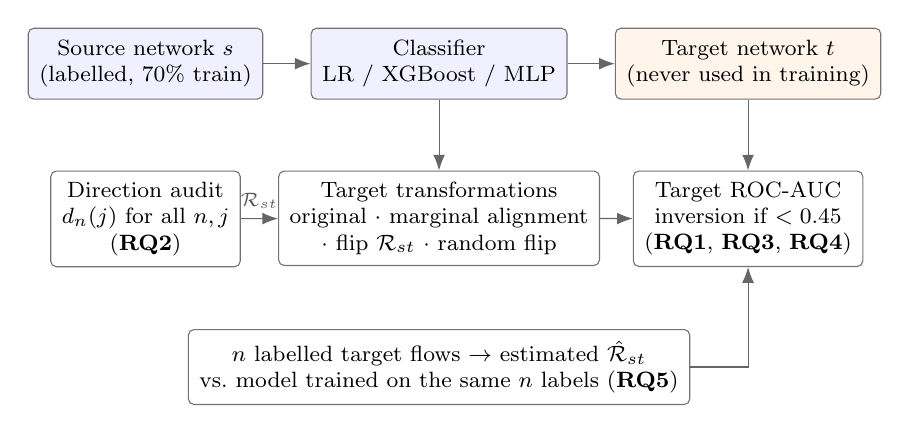
\begin{tikzpicture}[
  box/.style={draw=black!55, rounded corners=2pt, align=center, font=\footnotesize, inner sep=4pt, minimum height=9mm},
  lab/.style={font=\scriptsize, text=black!65},
  arr/.style={-{Latex[length=2mm]}, black!60}]
\node[box, fill=blue!6] (src) {Source network $s$\\(labelled, 70\% train)};
\node[box, fill=blue!6, right=6mm of src] (model) {Classifier\\LR / XGBoost / MLP};
\node[box, fill=orange!8, right=6mm of model] (tgt) {Target network $t$\\(never used in training)};
\node[box, below=9mm of src] (audit) {Direction audit\\$d_n(j)$ for all $n, j$\\(\RQ{2})};
\node[box, below=9mm of model] (inter) {Target transformations\\original $\cdot$ marginal alignment\\$\cdot$ flip $\mathcal{R}_{st}$ $\cdot$ random flip};
\node[box, below=9mm of tgt] (eval) {Target ROC-AUC\\inversion if $<0.45$\\(\RQ{1}, \RQ{3}, \RQ{4})};
\node[box, below=8mm of inter] (few) {$n$ labelled target flows $\rightarrow$ estimated $\hat{\mathcal{R}}_{st}$\\vs.\ model trained on the same $n$ labels (\RQ{5})};
\draw[arr] (src) -- (model);
\draw[arr] (model) -- (tgt);
\draw[arr] (tgt) -- (eval);
\draw[arr] (audit) -- node[lab, above]{$\mathcal{R}_{st}$} (inter);
\draw[arr] (inter) -- (eval);
\draw[arr] (model) -- (inter);
\draw[arr] (few) -| (eval);
\end{tikzpicture}
\caption{Study design. A detector trained on a source network is evaluated on every other network. The direction audit identifies features whose association with the attack label reverses between source and target; the oracle intervention transforms only the target features and keeps the trained detector fixed.}
\label{fig:design}
\end{figure}

Figure~\ref{fig:design} summarises the design. All code, configuration files and the scripts that generate every number, table and figure in this paper are available (see Data availability).

\subsection{Datasets and preprocessing}
\label{sec:data}

We use the NetFlow v2 versions of UNSW-NB15 (\net{UN}), CSE-CIC-IDS2018 (\net{CIC}), ToN-IoT (\net{TON}) and BoT-IoT (\net{BOT})~\cite{sarhan2022standard}, and, for \RQ{4}, their NetFlow v3 versions~\cite{luay2025temporal}. Table~\ref{tab:data} lists their sizes.

Features that identify endpoints or transactions were removed before any analysis: source and destination IPv4 addresses and ports, and \feat{DNS_QUERY_ID}, a transaction identifier. In NetFlow v3 we also removed the absolute flow start and end timestamps. Environment-dependent but semantically meaningful features such as \feat{MIN_TTL} and \feat{MAX_TTL} were retained, because whether they transfer is part of the question. This leaves \val{v2dos.nfeat} features in v2 and \val{v3dos.nfeat} in v3. Rows with missing or infinite values were removed; this affected only the v3 versions of \net{UN} (\val{v3dos.st.UN.nan} rows) and \net{BOT} (\val{v3dos.st.BOT.nan} rows). Exact duplicates over all remaining features, the label and the attack type were then removed.

Duplicate removal deserves a comment. With all original columns, records are essentially unique (at most \val{audit.dupall.max} duplicates). Once identifiers are dropped, however, many records become feature-identical---flooding attacks in particular produce large numbers of flows with the same statistics---so that, for example, \val{audit.BOT.dupnoiddns} of the \val{audit.BOT.raw} v2 \net{BOT} records duplicate another record. \feat{DNS_QUERY_ID} alone keeps many otherwise identical records apart: in v2 \net{UN}, \val{audit.UN.unoid} records are distinct with it and \val{audit.UN.unoiddns} without it. We therefore describe these as feature-identical rather than as erroneous duplicates; removing them prevents near-identical flows from appearing in both a training and a test split.

Continuous features that span several orders of magnitude (byte, packet, duration, throughput, window-size and inter-arrival-time features) were transformed with $\log(1+x)$ after clipping negative values at zero; categorical fields (protocol, application protocol, TCP flags, ICMP and DNS type codes) and TTLs were left unchanged. No other preprocessing was fitted to any data; standardisation for LR and MLP is part of each model pipeline and is fitted on the source training data only.

\begin{table}[t]
\centering
\caption{Datasets. \emph{Dup.}: share of records duplicating another record when all original columns are kept. \emph{Unique}: records after removing identifiers and feature-identical duplicates. \emph{Benign}, \emph{Attacks} (all attack types) and \emph{DoS/DDoS} are unique records; the benign and DoS/DDoS (or all-attack) records form the sampling pools of the aligned (binary) task. NetFlow v3 rows with missing or infinite values (\emph{NaN}) were removed first.}
\label{tab:data}
\footnotesize
\setlength{\tabcolsep}{3pt}
\begin{adjustbox}{max width=\textwidth}
\begin{tabular}{l rrrrrr rrrr}
\toprule
 & \multicolumn{6}{c}{NetFlow v2 (\val{v2dos.nfeat} features)} & \multicolumn{4}{c}{NetFlow v3 (\val{v3dos.nfeat} features)} \\
\cmidrule(lr){2-7}\cmidrule(lr){8-11}
Network & Flows & Dup.\,\% & Unique & Benign & Attacks & DoS/DDoS & Flows & NaN & Unique & DoS/DDoS \\
\midrule
\tabinput generated/tables/datasets.tex 
\bottomrule
\end{tabular}
\end{adjustbox}
\end{table}

\subsection{Tasks}
\label{sec:tasks}

The four benchmarks contain largely different attack types, so a model trained on one benchmark's attacks may simply never have seen the attacks of another. To remove this explanation we use an \emph{attack-family-aligned} task as the main protocol: benign flows against DoS and DDoS flows, the only family present in all four networks; other attack types are excluded. The DoS/DDoS classes are \net{UN}: DoS; \net{CIC}: the seven DoS and DDoS attack classes (Hulk, HOIC, GoldenEye, LOIC-HTTP, LOIC-UDP, Slowloris, SlowHTTPTest); \net{TON}: dos, ddos; \net{BOT}: DoS, DDoS. As a comparison we also use the conventional \emph{heterogeneous binary} task in which every attack type is positive. Both tasks are run on NetFlow v2; the aligned task is replicated on NetFlow v3.

\subsection{Sampling and transfer protocol}
\label{sec:protocol}

From the unique records of each network we draw a pool of at most 250{,}000 records per class. For each of five seeds, a balanced sample of up to 50{,}000 flows per class is drawn from the pool; where a class has fewer unique records (e.g.\ \val{v2dos.st.UN.pos} DoS flows in v2 \net{UN} and \val{v2dos.st.BOT.ben} benign flows in v2 \net{BOT}) all are used and the other class is subsampled to the same size. Seeds thus vary the data sample as well as the model initialisation.

For every source network and seed, the sample is split 70/30 (stratified). A classifier is trained on the 70\% and evaluated on the 30\% hold-out (in-domain) and on the full sample of every other network (cross-network). This gives 12 directed cross-network cells per classifier. We also train on the union of three networks and test on the fourth (leave-one-network-out). The target network contributes nothing to training, to feature processing or to any threshold.

\subsection{Classifiers}
\label{sec:clf}

We use three model families with fixed hyper-parameters, without tuning: L2-regularised logistic regression (LR) on standardised features; XGBoost~\cite{chen2016xgboost} with 300 trees of depth 6 and learning rate 0.1; and a multilayer perceptron (MLP) with hidden layers of 128 and 64 ReLU units, Adam and early stopping, on standardised features. LR and MLP use scikit-learn~\cite{pedregosa2011scikit}.

\subsection{Analyses}
\label{sec:analyses}

\paragraph{Transfer matrix and class swap (\RQ{1})}
We report target ROC-AUC for every cell. To ask whether inversion comes from the benign or the attack side, each single-source model is also evaluated on two mixed test sets: source hold-out benign with target attacks, and target benign with source hold-out attacks (equal class sizes). If replacing only one class by its target counterpart already reverses the ranking, that side's shift is sufficient to explain the inversion.

\paragraph{Direction audit (\RQ{2})}
For each network, seed and feature we compute $A_n(j)$ on the balanced sample and derive robust directions $d_n(j)$ and reversed sets $\mathcal{R}_{st}$ (Section~\ref{sec:defs}).

\paragraph{Oracle intervention (\RQ{2})}
For a model trained on $s$ and a target $t$, we keep the model fixed and transform the target features in four ways. \emph{Marginal alignment} maps each target feature through its own empirical distribution function onto the source training distribution, $x'_j = F^{-1}_{s,j}\!\left(\hat F_{t,j}(x_j)\right)$, using mid-ranks for ties; this uses no labels and makes every target marginal match the source. \emph{Alignment + flip} does the same but maps $\hat F_{t,j}(x_j)$ to $1-\hat F_{t,j}(x_j)$ for $j\in\mathcal{R}_{st}$, which reverses the order of exactly the reversed features while still matching the source marginals. \emph{Flip only} reverses the same features within the target's own distribution, without alignment. Finally, the \emph{random-flip control} applies alignment and reverses the same number of features drawn at random from those that are informative in both networks but not reversed (five draws, averaged). Only $\mathcal{R}_{st}$ depends on target labels; the intervention is therefore an oracle diagnostic of mechanism and not a deployable method.

\paragraph{Few-label direction estimation (\RQ{5})}
To ask how many target labels are needed to identify $\mathcal{R}_{st}$, we draw $n\in\{20,50,100,200,500\}$ labelled target flows ($n/2$ per class; 30 draws per seed), estimate target directions from these flows only, and apply alignment + flip to the remaining target flows (at most 20{,}000 per seed), which serve as the evaluation set. As a necessary baseline, LR and XGBoost (100 trees) are trained directly on the same $n$ labelled flows and evaluated on the same evaluation set.

\paragraph{Statistics}
We use two levels of analysis. The \emph{primary, descriptive} unit is a cell (training network $\times$ target network $\times$ classifier), averaged over seeds; all figures and the main tables report cells. Cells that share a training network are not independent, so we emphasise effect sizes: paired differences are summarised by their median and the matched-pairs rank-biserial correlation $r_{rb}$~\cite{kerby2014simple}; Wilcoxon signed-rank $p$-values~\cite{wilcoxon1945individual} are reported with Holm correction~\cite{holm1979simple} across the four comparisons in each table block. Means are given with 95\% bootstrap confidence intervals over cells (10{,}000 resamples). Because the three classifiers evaluated on the same network pair are the strongest source of dependence, inferential claims are additionally checked with a \emph{robustness} unit, the directed source--target network pair: classifier and seed results are averaged within each of the 12 directed pairs, and we report (i) the number of pairs in which one condition exceeds the other, (ii) a paired Wilcoxon signed-rank test across the 12 pair-averaged differences, and (iii) a 95\% interval for the mean difference over inverted cells obtained by a cluster bootstrap that resamples directed pairs rather than cells.

\paragraph{Implementation}
Experiments ran on an Apple M1 Ultra workstation with Python 3.12, NumPy 2.5, pandas 3.0, SciPy 1.18, scikit-learn 1.9 and XGBoost 3.4.

%% ===================================================================
\section{Results}
\label{sec:results}

\subsection{\RQ{1}: predictive inversion is common and robust}
\label{sec:rq1}

\begin{figure}[t]
\centering
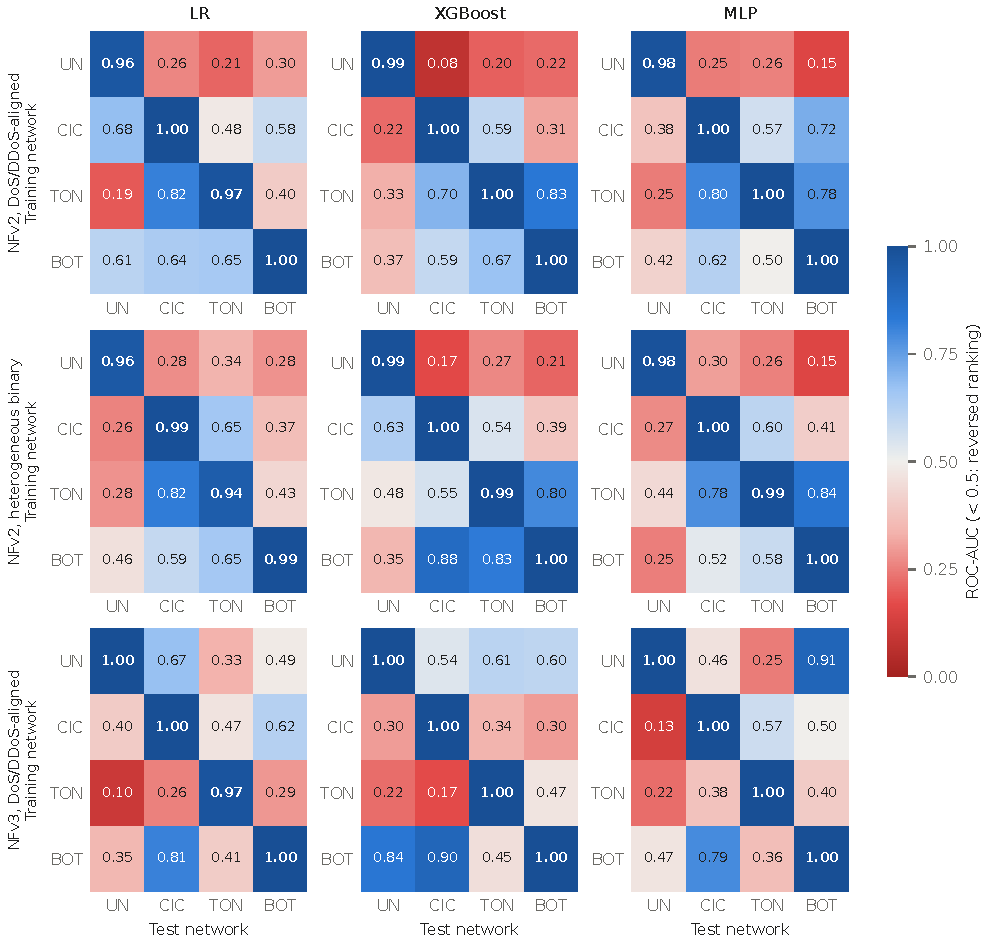
\includegraphics[width=\textwidth]{generated/figs/fig_transfer.pdf}
\caption{Single-source transfer matrices (ROC-AUC, mean over five seeds) for the three protocols (rows of panels: NetFlow v2 DoS/DDoS-aligned, NetFlow v2 heterogeneous binary, NetFlow v3 DoS/DDoS-aligned) and three classifiers (columns of panels). Within each panel, rows are the training network and columns the test network; the diagonal (bold) is the in-domain 30\% hold-out. \net{UN}: UNSW-NB15; \net{CIC}: CSE-CIC-IDS2018; \net{TON}: ToN-IoT; \net{BOT}: BoT-IoT. Red cells indicate ROC-AUC below 0.5, i.e.\ reversed ranking. The formal predictive-inversion criterion used in the analyses is mean ROC-AUC $<0.45$.}
\label{fig:transfer}
\end{figure}

\begin{table}[t]
\centering
\caption{In-domain versus cross-network ROC-AUC for single-source transfer (means over five seeds). \emph{In-domain}: mean and minimum over the four training networks; \emph{Cross AUC}: mean over the 12 directed cross-network cells. \emph{Inverted}: cells with mean AUC $<0.45$; \emph{All seeds $<0.5$}: cells in which every seed is below 0.5 (a different, not a stricter, criterion, so the two counts can differ in either direction). \emph{Lowest cell}: training$\rightarrow$test network (\net{UN}: UNSW-NB15; \net{CIC}: CSE-CIC-IDS2018; \net{TON}: ToN-IoT; \net{BOT}: BoT-IoT).}
\label{tab:model}
\footnotesize
\begin{adjustbox}{max width=\textwidth}
\begin{tabular}{llcccccl}
\toprule
Protocol & Model & \multicolumn{2}{c}{In-domain AUC} & Cross AUC & Inverted & All seeds & Lowest cell \\
 & & mean & min & mean & & $<0.5$ & \\
\midrule
\tabinput generated/tables/model_level.tex 
\bottomrule
\end{tabular}
\end{adjustbox}
\end{table}

Every model separated benign and DoS/DDoS traffic almost perfectly inside its own network: in-domain ROC-AUC ranged from \val{all.in.min} to \val{all.in.max} across all protocols and models (Table~\ref{tab:model}). Transfer to another network told a different story (Fig.~\ref{fig:transfer}). Under the attack-family-aligned NetFlow v2 task, \val{v2dos.rev.total} of \val{v2dos.ncells} single-source cells were inverted (LR \val{v2dos.lr.rev}, XGBoost \val{v2dos.xgboost.rev}, MLP \val{v2dos.mlp.rev} of 12), and in \val{v2dos.robust.total} cells every seed was below 0.5. The lowest value, \val{v2dos.xgboost.min} for XGBoost trained on \net{UN} and tested on \net{CIC}, means that the detector would rank a random benign flow above a random DoS flow in more than nine of ten pairs. Mean cross-network AUC was below 0.5 for every model (\val{v2dos.lr.crossmean}, \val{v2dos.xgboost.crossmean}, \val{v2dos.mlp.crossmean}).

Inversion did not depend on the model family: it occurred for the linear model, the tree ensemble and the neural network, often in the same cells (e.g.\ every model trained on \net{UN} was inverted on all three other networks). Training on three networks did not prevent it either: in leave-one-network-out transfer, \val{v2dos.lodo.below} of \val{v2dos.lodo.n} target $\times$ model combinations remained below 0.5 (minimum \val{v2dos.lodo.min}; Table~\ref{tab:lodo} in the Appendix).

Inversion was not the result of only one class moving. In the class-swap test (cell-level counts; Table~\ref{tab:swap} reports the pair-level means over models), among the \val{v2dos.swaprevn} inverted cells, replacing only the attack flows by target attacks reversed the ranking in \val{v2dos.swapattackside} cells and replacing only the benign flows did so in \val{v2dos.swapbenignside}; in the remaining \val{v2dos.swapbothabove} cells neither replacement alone was sufficient. The source model still separated target attacks from source benign flows, and source attacks from target benign flows, but placed target benign flows above target attacks. The score medians make this concrete: for models trained on \net{UN} and applied to \net{CIC}, the median attack score was \val{v2dos.pos.UN.CIC.tb} for target benign flows and \val{v2dos.pos.UN.CIC.ta} for target DoS flows (averaged over models). Across the 12 network pairs, target benign flows received the higher median score in \val{v2dos.pos.inv}, and in \val{v2dos.pos.coll} pairs both target classes received median scores below 0.05, so that a default threshold would detect almost nothing.

\subsection{\RQ{2}: inversion follows the reversal of feature--label directions}
\label{sec:rq2}

\begin{figure}[t]
\centering
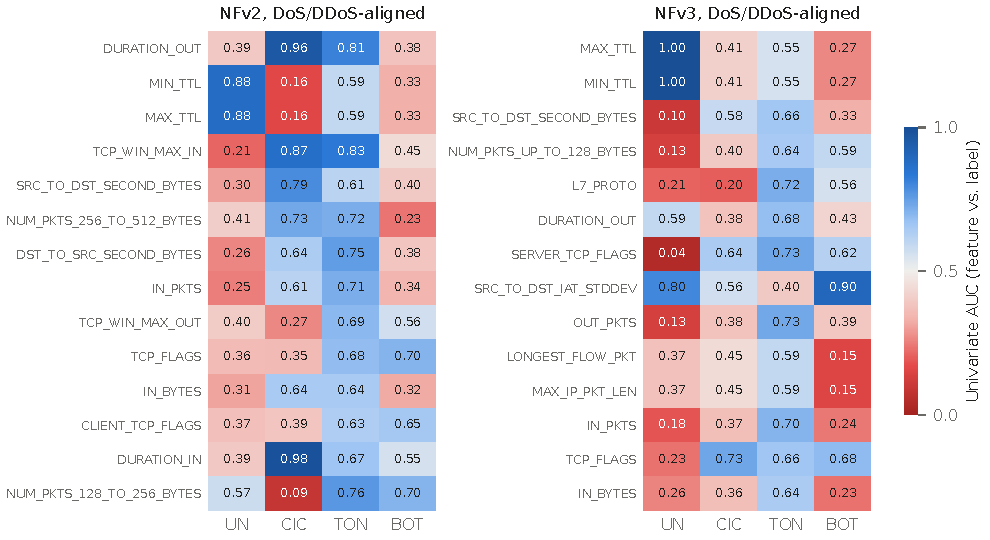
\includegraphics[width=\textwidth]{generated/figs/fig_features.pdf}
\caption{Univariate AUC of individual features in each network (mean over seeds) for the 14 features with the most reversed network pairs, in the three protocols. Blue ($A>0.5$): larger values indicate attacks; red ($A<0.5$): smaller values indicate attacks; white: uninformative. \net{UN}: UNSW-NB15; \net{CIC}: CSE-CIC-IDS2018; \net{TON}: ToN-IoT; \net{BOT}: BoT-IoT. Many features are strongly discriminative in every network but in opposite directions.}
\label{fig:features}
\end{figure}

\paragraph{Directions reverse for most features}
Figure~\ref{fig:features} shows the univariate AUC of the features with the most reversals. Of the \val{v2dos.f.nfeat} NetFlow v2 features, \val{v2dos.f.nrevany} were robustly reversed in at least one network pair under the aligned task. Among features informative in both networks of a pair, the share pointing in opposite directions ranged from \val{v2dos.f.prmin} to \val{v2dos.f.prmax} across the six pairs. The reversals concern ordinary flow statistics as well as environment-dependent fields. \feat{DURATION_OUT} indicated DoS when high in \net{CIC} ($A=\val{v2dos.fa.DURATION_OUT.CIC}$) and \net{TON} (\val{v2dos.fa.DURATION_OUT.TON}) but when low in \net{UN} (\val{v2dos.fa.DURATION_OUT.UN}) and \net{BOT} (\val{v2dos.fa.DURATION_OUT.BOT}); \feat{TCP_WIN_MAX_IN} was high for attacks in \net{CIC} and \net{TON} and low in \net{UN}; \feat{MIN_TTL} identified DoS by high values in \net{UN} ($A=\val{v2dos.fa.MIN_TTL.UN}$) and by low values in \net{CIC} (\val{v2dos.fa.MIN_TTL.CIC}).

\paragraph{The number of reversed features alone does not predict inversion}
Reversals were so widespread that every network pair had many, including pairs between which models transferred reasonably. Accordingly, the share of reversed features in a pair was not associated with the cross-network AUC of the 12 directed cells (Spearman $\rho=\val{v2dos.f.rho}$, $p=\val{v2dos.f.rhop}$). Whether a model inverts should depend on whether \emph{the features it relies on} reverse, which the count ignores. The intervention below tests this directly.

\begin{figure}[t]
\centering
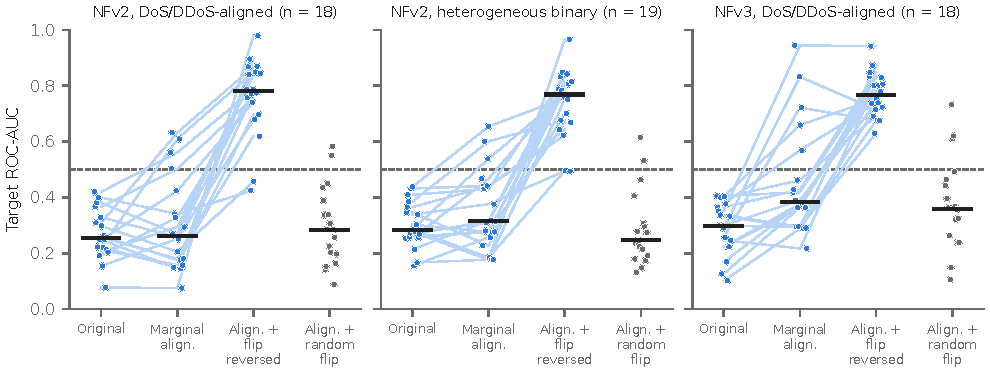
\includegraphics[width=\textwidth]{generated/figs/fig_oracle.pdf}
\caption{Oracle intervention on inverted cells (cross-network AUC $<0.45$; one point per training network $\times$ target network $\times$ model, mean over seeds; $n$: number of inverted cells per protocol). Lines connect the same cell; black bars are medians; dashed line: AUC $=0.5$. The flip-only condition is reported in Table~\ref{tab:oracle}. Marginal alignment matches every target feature distribution to the source; flipping additionally reverses only the features whose direction differs between source and target; the control reverses the same number of other informative features.}
\label{fig:oracle}
\end{figure}

\begin{table}[t]
\centering
\caption{Oracle intervention on inverted cells (training network $\times$ target network $\times$ classifier cells with seed-averaged AUC $<0.45$): mean target ROC-AUC [95\% bootstrap CI over cells] and number of cells restored above 0.5 (\emph{$>$.5}). The detector is fixed; only the target features are transformed. \emph{Marginal align.}: each target feature quantile-mapped onto the source distribution; \emph{Flip only}: features whose direction reversed between source and target are order-reversed without alignment; \emph{Align.\ + flip}: both; \emph{Align.\ + random flip}: alignment plus reversal of an equal number of other informative features (mean of five draws).}
\label{tab:oracle}
\scriptsize
\setlength{\tabcolsep}{2.5pt}
\begin{adjustbox}{max width=\textwidth}
\begin{tabular}{lc cc cc cc cc cc}
\toprule
Protocol & Cells & \multicolumn{2}{c}{Original} & \multicolumn{2}{c}{Marginal align.} & \multicolumn{2}{c}{Flip only} & \multicolumn{2}{c}{Align. + flip} & \multicolumn{2}{c}{Align. + random flip} \\
 & & AUC & $>$.5 & AUC & $>$.5 & AUC & $>$.5 & AUC & $>$.5 & AUC & $>$.5 \\
\midrule
\tabinput generated/tables/oracle.tex 
\bottomrule
\end{tabular}
\end{adjustbox}
\end{table}

\begin{table}[t]
\centering
\caption{Paired comparisons on inverted cells (seed-averaged AUC $<0.45$; conditions as in Table~\ref{tab:oracle}): median within-cell difference in target AUC (first condition minus second), matched-pairs rank-biserial correlation $r_{rb}$, and Wilcoxon signed-rank $p$, Holm-adjusted across the four comparisons within each protocol. Cells are not independent; see Table~\ref{tab:cluster} for the pair-level analysis.}
\label{tab:tests}
\footnotesize
\begin{adjustbox}{max width=\textwidth}
\begin{tabular}{llcccc}
\toprule
Protocol & Comparison & Cells & Median $\Delta$AUC & $r_{rb}$ & $p_{\mathrm{Holm}}$ \\
\midrule
\tabinput generated/tables/tests.tex 
\bottomrule
\end{tabular}
\end{adjustbox}
\end{table}

\paragraph{Correcting the reversed features restores the ranking}
Figure~\ref{fig:oracle} and Table~\ref{tab:oracle} show the intervention for the \val{v2dos.or.nrev} inverted cells of the aligned NetFlow v2 task. Matching every target marginal to the source left most cells inverted (mean AUC \val{v2dos.or.rev.base} before and \val{v2dos.or.rev.qmap} after alignment; median change \val{v2dos.t.rev.qmap-base.med}, $p_{\mathrm{Holm}}=\val{v2dos.t.rev.qmap-base.p}$), and restored only \val{v2dos.or.rest.qmap} cells above 0.5. When, in addition, the features in $\mathcal{R}_{st}$ were reversed, mean AUC rose to \val{v2dos.or.rev.qmapflip} [\val{v2dos.or.rev.qmapflip.lo}, \val{v2dos.or.rev.qmapflip.hi}] and \val{v2dos.or.rest.qmapflip} of \val{v2dos.or.nrev} cells exceeded 0.5. The gain over alignment alone was large and consistent (median \val{v2dos.t.rev.qmapflip-qmap.med}, $r_{rb}=\val{v2dos.t.rev.qmapflip-qmap.rrb}$, $p_{\mathrm{Holm}}=\val{v2dos.t.rev.qmapflip-qmap.p}$; Table~\ref{tab:tests}). Reversing the same number of other informative features did not help (\val{v2dos.or.rev.randflip}; \val{v2dos.or.rest.randflip} cells restored), so the recovery is specific to the features whose direction actually changed rather than a generic effect of perturbing the input. Flipping without alignment recovered part of the ranking (\val{v2dos.or.rev.flip}, \val{v2dos.or.rest.flip} cells), indicating that the reversal is the dominant factor but that marginal differences and the reversal interact. The conclusion does not rest on treating classifier-specific cells as independent. With directed network pairs as units, alignment + flip exceeded alignment alone in \val{v2dos.cl.qmapflip-qmap.ppos}/12 pairs in the aligned v2 task, \val{v2bin.cl.qmapflip-qmap.ppos}/12 in the binary v2 task and \val{v3dos.cl.qmapflip-qmap.ppos}/12 in v3, and the cluster-bootstrap intervals for the gain on inverted cells excluded zero in all three protocols ([\val{v2dos.cl.qmapflip-qmap.rlo}, \val{v2dos.cl.qmapflip-qmap.rhi}], [\val{v2bin.cl.qmapflip-qmap.rlo}, \val{v2bin.cl.qmapflip-qmap.rhi}] and [\val{v3dos.cl.qmapflip-qmap.rlo}, \val{v3dos.cl.qmapflip-qmap.rhi}]; Table~\ref{tab:cluster}). For the aligned v2 task, the pair-level median gain over alignment was \val{v2dos.cl.qmapflip-qmap.pmed} ($r_{rb}=\val{v2dos.cl.qmapflip-qmap.prrb}$, $p_{\mathrm{Holm}}=\val{v2dos.cl.qmapflip-qmap.pp}$), and alignment + flip exceeded the random control in \val{v2dos.cl.qmapflip-randflip.ppos} of \val{v2dos.cl.qmapflip-randflip.npairs} pairs.

On average \val{v2dos.or.nflip.mean} features were reversed per cell (range \val{v2dos.or.nflip.min}--\val{v2dos.or.nflip.max}). Recovery was substantial but not complete: corrected cells reached about 0.76 rather than the in-domain level of about 0.99, so differences beyond univariate direction---in magnitudes, interactions between features, or the attacks themselves---account for the remainder.

\subsection{\RQ{3}: task definition and direction threshold}
\label{sec:rq3}

\paragraph{Heterogeneous binary task}
Aligning the attack family did not reduce inversion. Under the heterogeneous binary task, \val{v2bin.rev.total} of \val{v2bin.ncells} cells were inverted, compared with \val{v2dos.rev.total} under the aligned task (Table~\ref{tab:model}), and the intervention reproduced the aligned result: alignment alone gave \val{v2bin.or.rev.qmap} (\val{v2bin.or.rest.qmap} of \val{v2bin.or.nrev} restored), alignment + flip \val{v2bin.or.rev.qmapflip} (\val{v2bin.or.rest.qmapflip} restored), and the random control \val{v2bin.or.rev.randflip} (\val{v2bin.or.rest.randflip} restored). In this task, alignment alone produced a small improvement on inverted cells (median \val{v2bin.t.rev.qmap-base.med}, $p_{\mathrm{Holm}}=\val{v2bin.t.rev.qmap-base.p}$; not significant with directed network pairs as units, Table~\ref{tab:cluster}), much smaller than that of the targeted flip (median \val{v2bin.t.rev.qmapflip-qmap.med} over alignment, $r_{rb}=\val{v2bin.t.rev.qmapflip-qmap.rrb}$). Mismatched attack types therefore do not account for inversion on these benchmarks.

\begin{table}[t]
\centering
\caption{Sensitivity of the oracle intervention to the direction thresholds $\tau_{\mathrm{hi}}/\tau_{\mathrm{lo}}$: mean number of flipped features per cell, mean AUC of inverted cells after alignment + flip and after alignment + random flip, and cells restored above 0.5 (restored/inverted). The 0.55/0.45 row corresponds to Table~\ref{tab:oracle}; the random features were redrawn independently in this analysis, so the random-flip values in that row differ slightly from Table~\ref{tab:oracle}.}
\label{tab:sens}
\footnotesize
\begin{adjustbox}{max width=\textwidth}
\begin{tabular}{llccccc}
\toprule
Protocol & $\tau_{\mathrm{hi}}/\tau_{\mathrm{lo}}$ & Flipped & \multicolumn{2}{c}{Align. + flip} & \multicolumn{2}{c}{Random flip} \\
 & & features & AUC & restored & AUC & restored \\
\midrule
\tabinput generated/tables/sensitivity.tex 
\bottomrule
\end{tabular}
\end{adjustbox}
\end{table}

\paragraph{Direction threshold}
Calling a direction at $0.52/0.48$, $0.55/0.45$ or $0.60/0.40$ changed the number of flipped features (Table~\ref{tab:sens}) but not the conclusion: alignment + flip restored \val{v2dos.sens.restmin}--\val{v2dos.sens.restmax} of the \val{v2dos.or.nrev} inverted cells in the aligned task and \val{v2bin.sens.restmin}--\val{v2bin.sens.restmax} of \val{v2bin.or.nrev} in the binary task, whereas the random control never restored more than \val{v2bin.sens.rfmax}.

\subsection{\RQ{4}: replication with NetFlow v3}
\label{sec:rq4}

NetFlow v3 adds inter-arrival-time features and is produced by a newer extraction pipeline from the same four testbeds; it therefore tests whether the findings depend on the v2 representation, not whether they hold in new networks. All findings replicated (Fig.~\ref{fig:transfer}, Tables~\ref{tab:model}--\ref{tab:sens}). In-domain AUC was at least \val{v3dos.in.min}; \val{v3dos.rev.total} of \val{v3dos.ncells} cells were inverted, with values as low as \val{v3dos.cross.min}; and in leave-one-network-out transfer all \val{v3dos.lodo.below} target $\times$ model combinations were below 0.5. \val{v3dos.f.nrevany} of \val{v3dos.f.nfeat} features were reversed in at least one pair. TTL was a striking case: \feat{MIN_TTL} separated DoS from benign traffic perfectly in v3 \net{UN} ($A=\val{v3dos.fa.MIN_TTL.UN}$) but pointed the other way in \net{BOT} (\val{v3dos.fa.MIN_TTL.BOT}), and \feat{SERVER_TCP_FLAGS} was nearly perfectly reversed in \net{UN} (\val{v3dos.fa.SERVER_TCP_FLAGS.UN}) relative to the other three networks.

The intervention restored \val{v3dos.or.rest.qmapflip} of \val{v3dos.or.nrev} inverted cells (mean \val{v3dos.or.rev.qmapflip} [\val{v3dos.or.rev.qmapflip.lo}, \val{v3dos.or.rev.qmapflip.hi}]), against \val{v3dos.or.rest.randflip} for the random control (\val{v3dos.or.rev.randflip}). One difference from v2 should be noted: in v3, marginal alignment alone helped more (mean \val{v3dos.or.rev.base} $\rightarrow$ \val{v3dos.or.rev.qmap}; median change \val{v3dos.t.rev.qmap-base.med}, $p_{\mathrm{Holm}}=\val{v3dos.t.rev.qmap-base.p}$), so marginal shift contributes to inversion in this representation. The targeted flip nevertheless added a large further gain (median \val{v3dos.t.rev.qmapflip-qmap.med} over alignment, $r_{rb}=\val{v3dos.t.rev.qmapflip-qmap.rrb}$, $p_{\mathrm{Holm}}=\val{v3dos.t.rev.qmapflip-qmap.p}$), which held in \val{v3dos.cl.qmapflip-qmap.ppos} of \val{v3dos.cl.qmapflip-qmap.npairs} directed network pairs when classifiers were averaged (Table~\ref{tab:cluster}). Unlike in v2, the share of reversed features in a pair was associated with cross-network AUC in v3 ($\rho=\val{v3dos.f.rho}$, $p=\val{v3dos.f.rhop}$); with only 12 directed cells per protocol and no association in either v2 protocol (aligned $\rho=\val{v2dos.f.rho}$, binary $\rho=\val{v2bin.f.rho}$), we do not interpret this pair-level correlation further.

\subsection{\RQ{5}: few labels identify the reversals, but local training is better}
\label{sec:rq5}

\begin{figure}[t]
\centering
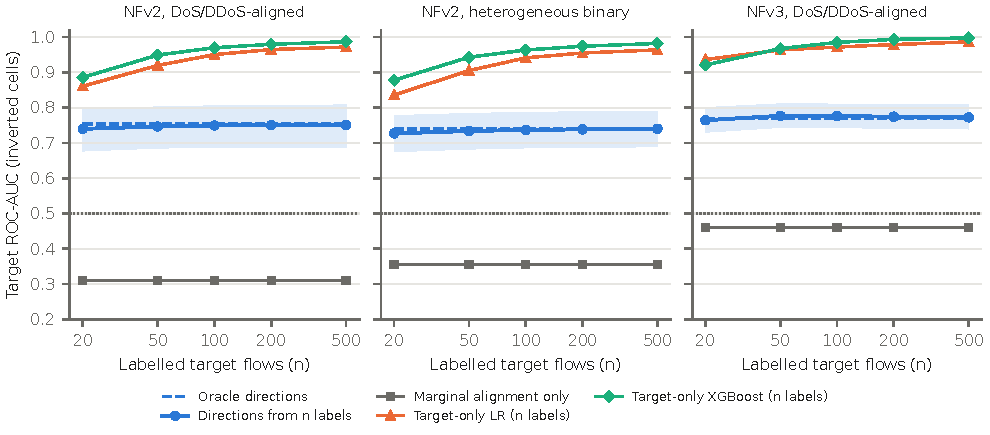
\includegraphics[width=\textwidth]{generated/figs/fig_fewlabel.pdf}
\caption{Inverted cells: target AUC when the reversed features are estimated from $n$ class-balanced labelled target flows ($n/2$ benign and $n/2$ attack) (shaded: 95\% bootstrap CI over cells), compared with oracle directions, marginal alignment alone, and LR and XGBoost trained only on the same $n$ labelled flows. Inverted cells: seed-averaged single-source AUC $<0.45$. Each point averages 30 label draws per seed. The $n$ labelled flows are excluded from the evaluation set (at most 20{,}000 remaining target flows per seed); dotted line: AUC $=0.5$.}
\label{fig:fewlabel}
\end{figure}

\begin{table}[t]
\centering
\caption{Few-label direction estimation on inverted cells: precision and recall of the estimated reversed-feature set relative to the oracle set, target AUC after alignment + flip with estimated and oracle directions, and AUC of models trained only on the $n$ class-balanced labelled target flows ($n/2$ per class; 30 draws per seed). All AUCs are computed on inverted cells (seed-averaged AUC $<0.45$) and on the evaluation flows that remain after removing the $n$ labelled flows; the oracle value therefore differs slightly from Table~\ref{tab:oracle}, which uses the full target sample.}
\label{tab:few}
\footnotesize
\begin{adjustbox}{max width=\textwidth}
\begin{tabular}{llcccccc}
\toprule
Protocol & $n$ & Precision & Recall & Estimated & Oracle & Target-only & Target-only \\
 & & & & flip AUC & flip AUC & LR & XGBoost \\
\midrule
\tabinput generated/tables/fewlabel.tex 
\bottomrule
\end{tabular}
\end{adjustbox}
\end{table}

Reversed features were easy to identify from few labels (Fig.~\ref{fig:fewlabel}, Table~\ref{tab:few}). With $n=20$ labelled target flows (ten benign and ten DoS/DDoS), the estimated reversed set had a precision of \val{v2dos.few.20.prec} and a recall of \val{v2dos.few.20.rec} relative to the oracle set in the aligned v2 task, and alignment + flip with these estimated directions reached \val{v2dos.few.20.est} against \val{v2dos.few.20.oracle} with oracle directions on the same evaluation flows. At $n=50$, precision and recall were \val{v2dos.few.50.prec} and \val{v2dos.few.50.rec}. The same held in the binary task and in v3.

The same labels, however, were better spent on a local model. LR and XGBoost trained only on the $n=20$ labelled target flows reached \val{v2dos.few.20.tolr} and \val{v2dos.few.20.toxgb} on the evaluation flows of the inverted cells, and \val{v2dos.few.50.tolr} and \val{v2dos.few.50.toxgb} with $n=50$, well above any corrected source model (v3: \val{v3dos.few.20.tolr} and \val{v3dos.few.20.toxgb} at $n=20$). Within each network the classes are nearly separable, so a handful of local examples is enough. The value of the correction lies in what it reveals about the source model, not in its use as an adaptation method. Note that this experiment measures label efficiency conditional on having examples of both classes: it does not imply that twenty randomly sampled operational flows, which at realistic attack prevalence would rarely contain any attack, would suffice.

%% ===================================================================
\section{Discussion}
\label{sec:discussion}

\paragraph{What inverts, and why}
The results are consistent with a specific explanation. On these benchmarks, marginal distribution shift alone did not account for inversion. Its contribution depends on the representation: matching every target marginal to the source changed inverted cells little in NetFlow v2 but recovered part of the ranking in NetFlow v3; in all three protocols, correcting reversed feature--label directions produced a substantially larger additional recovery. Nor did mismatched attack types account for it: holding the attack family fixed produced as much inversion as the heterogeneous task. Nor was it attributable to one class alone: in most inverted cells neither the benign nor the attack side alone reversed the ranking. The explanation best supported by our analyses is that many features separate DoS from benign traffic in opposite directions in different networks, and that a model trained in one network carries those directions into another. Reversing exactly those features, and no others, restored most rankings, although only to an AUC of about 0.74--0.77 rather than the in-domain level: correcting direction reversals recovers a large fraction, but not all, of the lost ranking. In the terms of the dataset-shift taxonomy, this is a shift in class-conditional feature relationships that is consistent with concept shift~\cite{gama2014survey,morenotorres2012unifying}, and of a structured kind: not a weakening of the feature--label relationship, but its reversal.

The pair-level analyses add a qualification. The share of reversed features in a network pair was unrelated to cross-network AUC in both NetFlow v2 protocols but correlated with it in v3, whereas the targeted intervention worked consistently in all three. The prevalence of reversed features is therefore not a representation-invariant predictor of failure; our results suggest that which relationships a model relies on matters more than how many relationships reverse, although we did not measure model reliance directly.

Some of the reversed features plausibly encode how each testbed was built rather than what the attacks do. TTL values depend on operating systems and on the number of hops between attack generators and victims; in v3 \net{UN}, TTL alone separated DoS and benign traffic perfectly. Durations, window sizes and packet-size bins depend on the tools used to generate both the attacks and the benign background. A model that learns such regularities may learn properties of the testbed rather than of the attacks~\cite{geirhos2020shortcut,arp2022dos}. Our direction audit does not distinguish artefacts from genuine differences in attack behaviour between networks, and it does not need to: either way, for the reversed features, the relationship that a detector learns in one network does not hold in another.

\paragraph{Implications for evaluation}
Three practical consequences follow. First, cross-network results should be reported with threshold-free ranking metrics alongside detection rates. In \val{v2dos.pos.coll} of the 12 directed pairs of the aligned v2 task, both target classes received median attack scores below 0.05, so detection-rate-based results would show near-zero detection and hide whether the ranking was merely shifted or inverted. Second, a direction audit of the kind used here is cheap, requires labels in both networks but no model, and shows before any training whether two benchmarks agree on how their features relate to the label; substantial disagreement in feature directions should be treated as a warning sign for cross-network transfer, although transferability ultimately depends on which features and interactions a particular model relies on. Third, in our experiments pooling three source networks did not remove inversion: leave-one-network-out models remained below chance in \val{v2dos.lodo.below} of \val{v2dos.lodo.n} target $\times$ model combinations in v2 and in \val{v3dos.lodo.below} of \val{v3dos.lodo.n} in v3, consistent with pooled data containing contradictory directions.

\paragraph{Implications for deployment}
Domain-adaptation methods that rely primarily on marginal distribution alignment~\cite{sun2016return} cannot, by marginal matching alone, resolve a feature--label relationship whose direction itself has changed; our quantile-mapping condition isolates this marginal-alignment component and recovered at most part of the lost ranking. Methods that also align class-conditional structure or adapt with target labels or pseudo-labels~\cite{ganin2016domain} are not covered by this conclusion and would need to be evaluated directly. The few-label experiment suggests a sober operational conclusion: in our experiments, once even a very small labelled sample containing both classes was available for a target network, a locally trained detector outperformed the transferred one, which matters because the transferred model is not merely uninformative but can be actively misleading. Obtaining confirmed attack examples in an operational network is itself costly, and our experiment does not quantify that cost.

\paragraph{Threats to validity}
The intervention is an oracle: $\mathcal{R}_{st}$ is determined with target labels, and the intervention shows that correcting these features suffices to restore most rankings, not that they are the only cause or that the correction is deployable. The univariate direction ignores interactions, and recovery was partial. The four benchmarks and their NetFlow v2 and v3 versions come from four testbeds; NetFlow v3 shows that the findings are not tied to one extraction pipeline, not that they hold in other networks. The DoS/DDoS family covers different attack implementations across benchmarks (e.g.\ HTTP floods in \net{CIC}, network-layer floods in \net{BOT}), so ``aligned'' means the same family, not the same attack tool. Unique DoS records were few in \net{UN} (\val{v2dos.st.UN.pos} in v2), so samples for this network overlapped across seeds. Finally, the 36 cells per protocol share training networks and are not independent; we therefore report effect sizes and confidence intervals alongside $p$-values, repeat the key tests with directed network pairs as units and a cluster bootstrap, and our conclusions rest on the size and consistency of the effects across three protocols, three models and three thresholds rather than on any single test.

%% ===================================================================
\section{Conclusion}
\label{sec:conclusion}

NIDS models that were nearly perfect in one benchmark network frequently inverted their ranking in another, even when the attack family is the same and the training data come from several networks. Our analyses link much of this inversion to the features themselves: most NetFlow features discriminated attacks in opposite directions in at least one pair of networks, and reversing only those features restored most inverted rankings, whereas matching marginal distributions recovered far less. The finding held for linear, tree-based and neural models, for an aligned and a heterogeneous task, for NetFlow v2 and v3, and across direction thresholds. For research, it argues for auditing the direction of feature--label relationships before treating benchmarks as interchangeable domains. For practice, it argues for training on a small, class-balanced local sample, where one can be obtained, rather than transferring a benchmark-trained detector. Future work should examine whether direction reversals also occur in operational networks and whether they can be detected from unlabelled traffic.

%% ===================================================================
\section*{CRediT authorship contribution statement}

\textbf{Haoyu Zhang}: Conceptualization, Methodology, Software,
Formal analysis, Investigation, Data curation,
Writing -- original draft, Visualization.

\textbf{Mei Wang}: Conceptualization, Methodology,
Validation, Writing -- review \& editing,
Supervision, Project administration.

\section*{Declaration of competing interest}
The authors declare no known competing financial interests or personal relationships that could have appeared to influence the work reported in this paper.

\section*{Funding}

This work was supported by the Sichuan Provincial Department of Education (Third Batch of Curriculum Ideological and Political Education Demonstration Course Program, Computer Networks) and the Teaching Guidance Committee for College Computer Courses of the Ministry of Education of China [grant number AIGE-202409]. 

\section*{Data availability}
%% TODO(author): add the repository / Zenodo DOI.
The NetFlow datasets are publicly available from the University of Queensland. All code, configuration files, per-run results and the scripts that generate every number, table and figure in this paper will be made available at \textit{[repository URL / DOI]}.

\section*{Declaration of generative AI and AI-assisted technologies in the manuscript preparation process}

During the preparation of this work, the authors used Claude(Anthropic) to improve language, readability, and clarity. After using this tool, the authors reviewed and edited the content as needed and take full responsibility for the content of the publication.

%% ===================================================================
\appendix
\section{Additional results}
\label{app:extra}

\begin{table}[h]
\centering
\caption{Leave-one-network-out transfer: target ROC-AUC (mean over five seeds) when training on the union of the other three networks. NFv2/NFv3: NetFlow v2/v3; DoS/DDoS: attack-family-aligned task; binary: heterogeneous binary task; XGB: XGBoost. Values below 0.5 indicate reversed ranking.}
\label{tab:lodo}
\footnotesize
\begin{adjustbox}{max width=\textwidth}
\begin{tabular}{l ccc ccc ccc}
\toprule
 & \multicolumn{3}{c}{NFv2, DoS/DDoS} & \multicolumn{3}{c}{NFv2, binary} & \multicolumn{3}{c}{NFv3, DoS/DDoS} \\
\cmidrule(lr){2-4}\cmidrule(lr){5-7}\cmidrule(lr){8-10}
Target & LR & XGB & MLP & LR & XGB & MLP & LR & XGB & MLP \\
\midrule
\tabinput generated/tables/lodo.tex 
\bottomrule
\end{tabular}
\end{adjustbox}
\end{table}

\begin{table}[h]
\centering
\caption{Class-swap decomposition (ROC-AUC, mean over models and seeds). \emph{Cross}: target benign vs.\ target attacks. \emph{T.att.}: source benign vs.\ target attacks. \emph{T.ben.}: target benign vs.\ source attacks. Source flows are the source hold-out; classes are balanced. A value below 0.5 in \emph{T.att.} (\emph{T.ben.}) means that replacing only the attack (benign) class by its target counterpart already reverses the ranking. Transfer: training$\rightarrow$test network (\net{UN}: UNSW-NB15; \net{CIC}: CSE-CIC-IDS2018; \net{TON}: ToN-IoT; \net{BOT}: BoT-IoT); NFv2/NFv3: NetFlow v2/v3.}
\label{tab:swap}
\scriptsize
\setlength{\tabcolsep}{3pt}
\begin{adjustbox}{max width=\textwidth}
\begin{tabular}{l ccc ccc ccc}
\toprule
 & \multicolumn{3}{c}{NFv2, DoS/DDoS} & \multicolumn{3}{c}{NFv2, binary} & \multicolumn{3}{c}{NFv3, DoS/DDoS} \\
\cmidrule(lr){2-4}\cmidrule(lr){5-7}\cmidrule(lr){8-10}
Transfer & Cross & T.att. & T.ben. & Cross & T.att. & T.ben. & Cross & T.att. & T.ben. \\
\midrule
\tabinput generated/tables/swap.tex 
\bottomrule
\end{tabular}
\end{adjustbox}
\end{table}

\begin{table}[h]
\centering
\caption{Robustness of the oracle comparisons to dependence between cells. Each unit is one directed source--target network pair after averaging over classifiers and seeds (12 pairs per protocol). \emph{Pairs $>0$}: number of pairs with a positive difference. Median $\Delta$AUC, $r_{rb}$ and $p_{\mathrm{Holm}}$: paired Wilcoxon signed-rank test across the 12 pair-averaged differences, Holm-adjusted within each protocol. Comparisons as in Table~\ref{tab:tests}. \emph{Cluster bootstrap}: mean difference over inverted cells (seed-averaged cell AUC $<0.45$) with a 95\% interval obtained by resampling directed network pairs (10{,}000 resamples).}
\label{tab:cluster}
\footnotesize
\begin{adjustbox}{max width=\textwidth}
\begin{tabular}{llccccc}
\toprule
Protocol & Comparison & Pairs $>0$ & Median $\Delta$AUC & $r_{rb}$ & $p_{\mathrm{Holm}}$ & Cluster bootstrap (inverted cells) \\
\midrule
\tabinput generated/tables/cluster.tex 
\bottomrule
\end{tabular}
\end{adjustbox}
\end{table}
\clearpage

\bibliographystyle{elsarticle-num}
\bibliography{refs}

\end{document}
